%----------------------------------------------------------------------------------------
%	Capítulo 3
%----------------------------------------------------------------------------------------

\pagestyle{myportland}
\doublespacing
%\pagenumbering{arabic}
\chapter[----- Diseño Mecatrónico]{Diseño Mecatrónico}
\thispagestyle{myportland}

%% NUEVA SECCIÓN X.X
\section{Desarrollo de proyecto conceptual}

El diseño conceptual es parte del proceso de diseño en la que --mediante la identificación de problemas esenciales a través de la abstracción, el establecimiento de estructuras funcionales, búsqueda de principios de funcionamiento adecuados y su combinación en una estructura global-- se establece a través de la elaboración de un principio de solución.\cite[p.~159]{Pahl2007}

%% NUEVO SUBSECCION X.X.X
\subsection{Lista de requerimientos}

La lista de requerimientos (Tabla \ref{tab:resumen de los requerimientos del sistema}) se formuló mediante la realización de entrevistas (Anexo  A1) en las cuales se recopilaron aspectos requerimientos implícitos y explícitos de calidad y cantidad que debe tener el sistema en general. Dicha entrevista se planteó con las recomendaciones que muestra el libro \textit{Engineering Design}\footnote{Engineering Design – A Systematic Approach.\cite[p.~144-158]{Pahl2007}}.

\begin{savenotes}
	% Please add the following required packages to your document preamble:
	% \usepackage{multirow}
	% \usepackage[table,xcdraw]{xcolor}
	% If you use beamer only pass "xcolor=table" option, i.e. \documentclass[xcolor=table]{beamer}
	% \usepackage{longtable}
	% Note: It may be necessary to compile the document several times to get a multi-page table to line up properly
	\scriptsize
	\begin{longtable}{|c|p{0.6cm}|p{10cm}|c|}		
		\caption{Resumen de los requerimientos del sistema.}
		\label{tab:resumen de los requerimientos del sistema}\\
		\hline
		\rowcolor[HTML]{A6A6A6} 
		\multicolumn{4}{|c|}{\cellcolor[HTML]{A6A6A6}{\color[HTML]{000000} \textbf{LISTA DE REQUERIMIENTOS}}} \\ \hline
		\endfirsthead
		%
		\multicolumn{4}{c}%
		{{Tabla \thetable\ continuación de la anterior página.}} \\
		\hline
		\rowcolor[HTML]{A6A6A6} 
		\multicolumn{4}{|c|}{\cellcolor[HTML]{A6A6A6}{\color[HTML]{000000} \textbf{LISTA DE REQUERIMIENTOS}}} \\ \hline
		\rowcolor[HTML]{D9D9D9} 
		\textbf{PROYECTO} &
		\multicolumn{2}{c|}{\cellcolor[HTML]{D9D9D9}\textbf{\begin{tabular}[c]{@{}c@{}}DISEÑO DE CLASIFICADORA Y CONTADORA\\  DE TRUCHAS ARCOÍRIS (Oncorhynchus mykiss)\\ DE 10 A 20 CM. PARA LA CRIANZA DE TRUCHAS\\ EN LA LAGUNA DE PAUCARCOCHA\end{tabular}}} &
		\textbf{\begin{tabular}[c]{@{}c@{}}Fecha:\\ 2020-05-07\\ Página 1 de 1\end{tabular}} \\ \hline
		\rowcolor[HTML]{D9D9D9} 
		{\color[HTML]{000000} \textbf{\begin{tabular}[c]{@{}c@{}}Última \\ modificación\end{tabular}}} &
		{\color[HTML]{000000} \textbf{\begin{tabular}[c]{@{}c@{}}D/\\ E\end{tabular}}} &
		\multicolumn{1}{c|}{\cellcolor[HTML]{D9D9D9}{\color[HTML]{000000} \textbf{Requerimientos}}} &
		{\color[HTML]{000000} \textbf{Reponsable}} \\ \hline
		\endhead
		%
		\rowcolor[HTML]{D9D9D9} 
		\textbf{PROYECTO} &
		\multicolumn{2}{c|}{\cellcolor[HTML]{D9D9D9}\textbf{\begin{tabular}[c]{@{}c@{}}DISEÑO DE CLASIFICADORA Y CONTADORA\\  DE TRUCHAS ARCOÍRIS (Oncorhynchus mykiss)\\ DE 10 A 20 CM. PARA LA CRIANZA DE TRUCHAS\\ EN LA LAGUNA DE PAUCARCOCHA\end{tabular}}} &
		\textbf{\begin{tabular}[c]{@{}c@{}}Fecha:\\ 2020-05-07\\ Página 1 de 1\end{tabular}} \\ \hline
		\rowcolor[HTML]{D9D9D9} 
		{\color[HTML]{000000} \textbf{\begin{tabular}[c]{@{}c@{}}Última \\ modificación\end{tabular}}} &
		{\color[HTML]{000000} \textbf{\begin{tabular}[c]{@{}c@{}}D/E\footnote{Deseo (D) y exigencia (E).}\end{tabular}}} &
		\multicolumn{1}{c|}{\cellcolor[HTML]{D9D9D9}{\color[HTML]{000000} \textbf{Requerimientos}}} &
		{\color[HTML]{000000} \textbf{Reponsable}} \\ \hline
		
		
		&    & \underline{Función principal:}																										& P.D.V. 	\\
		2019-09-24  & E  & Clasificar y contar truchas arcoíris de 10 a 20 $ cm $. en al menos 2 salidas y enviar un reporte de la clasificación y el conteo.   & \multicolumn{1}{l|}{}	\\ 
		&    & \underline{Geometría:}																												& \multicolumn{1}{l|}{}	\\
		2019-09-24  & E  & El sistema no debe exceder los 200x200x200 $ cm $.																					& \multicolumn{1}{l|}{}	\\ 
		&    & \underline{Fuerzas:}																													& \multicolumn{1}{l|}{}	\\
		2019-09-24  & E  & Pesar menos de 200 $ kg $.																											& \multicolumn{1}{l|}{}	\\ 
		&    & \underline{Energía:}																													& \multicolumn{1}{l|}{}	\\
		2019-10-05  & E  & Usará baterías DC.																													& \multicolumn{1}{l|}{}	\\ 	
		2019-09-24  & E  & Funcionar desde -10 a 40 °C.																											& \multicolumn{1}{l|}{}	\\ 	
		2019-09-24  & D  & La máquina debe enviar la información.																								& \multicolumn{1}{l|}{}	\\ 	
		&    & \underline{Materiales:}																												& \multicolumn{1}{l|}{}	\\
		2019-09-22  & E  & La máquina debe ser inoxidable.																										& \multicolumn{1}{l|}{}	\\ 	
		2019-09-20  & E  & La máquina no debe desprender ningún residuo que pueda contaminar el agua.															& \multicolumn{1}{l|}{}	\\ 	
		2019-09-25  & D  & Los materiales de manufactura deben poder ser adquiridos en el mercado peruano.														& \multicolumn{1}{l|}{}	\\ 			
		&    & \underline{Señales:}																													& \multicolumn{1}{l|}{}	\\
		2019-09-24  & E  & Se debe enviar una señal en caso de fallo del sistema y pausar el proceso.															& \multicolumn{1}{l|}{}	\\ 	
		&    & \underline{Hardware:}																												& \multicolumn{1}{l|}{}	\\
		2019-10-05  & E  & La máquina debe usar cámaras o dispositivos similares para obtener imágenes.															& \multicolumn{1}{l|}{}	\\ 		
		&    & \underline{Software:}																												& \multicolumn{1}{l|}{}	\\
		2019-10-05  & D  & El sistema generará un reporte de la clasificación y conteo.																			& \multicolumn{1}{l|}{}	\\ 	
		&    & \underline{Costos:}   																												& \multicolumn{1}{l|}{}	\\ 
		2019-09-24  & D  & El precio unitario menor a 10 mil dólares.       								    												& \multicolumn{1}{l|}{}	\\  \hline
		
		
		\rowcolor[HTML]{D9D9D9} 
		\multicolumn{1}{|l|}{\cellcolor[HTML]{D9D9D9}{\color[HTML]{000000} }} &
		\multicolumn{2}{c|}{\cellcolor[HTML]{D9D9D9}{\color[HTML]{000000} \textbf{Última modificación: 2019-10-05}}} &
		{\color[HTML]{000000} } \\ \hline
	\end{longtable}
	
\end{savenotes}

%% NUEVO SUBSECCION X.X.X
\subsection{Caja negra}

La caja negra mostrada en la Figura \ref{fig:caja negra del sistema} representa la energía (flecha continua), materia (flecha gruesa) y señales (flecha discontinua) que necesita y brinda el sistema para funcionar como un sistema clasificador y contador de truchas de un determinado rango según la lista de requerimientos mostrada en la Tabla \ref{tab:resumen de los requerimientos del sistema}.

\begin{figure}[H]
	\centering
	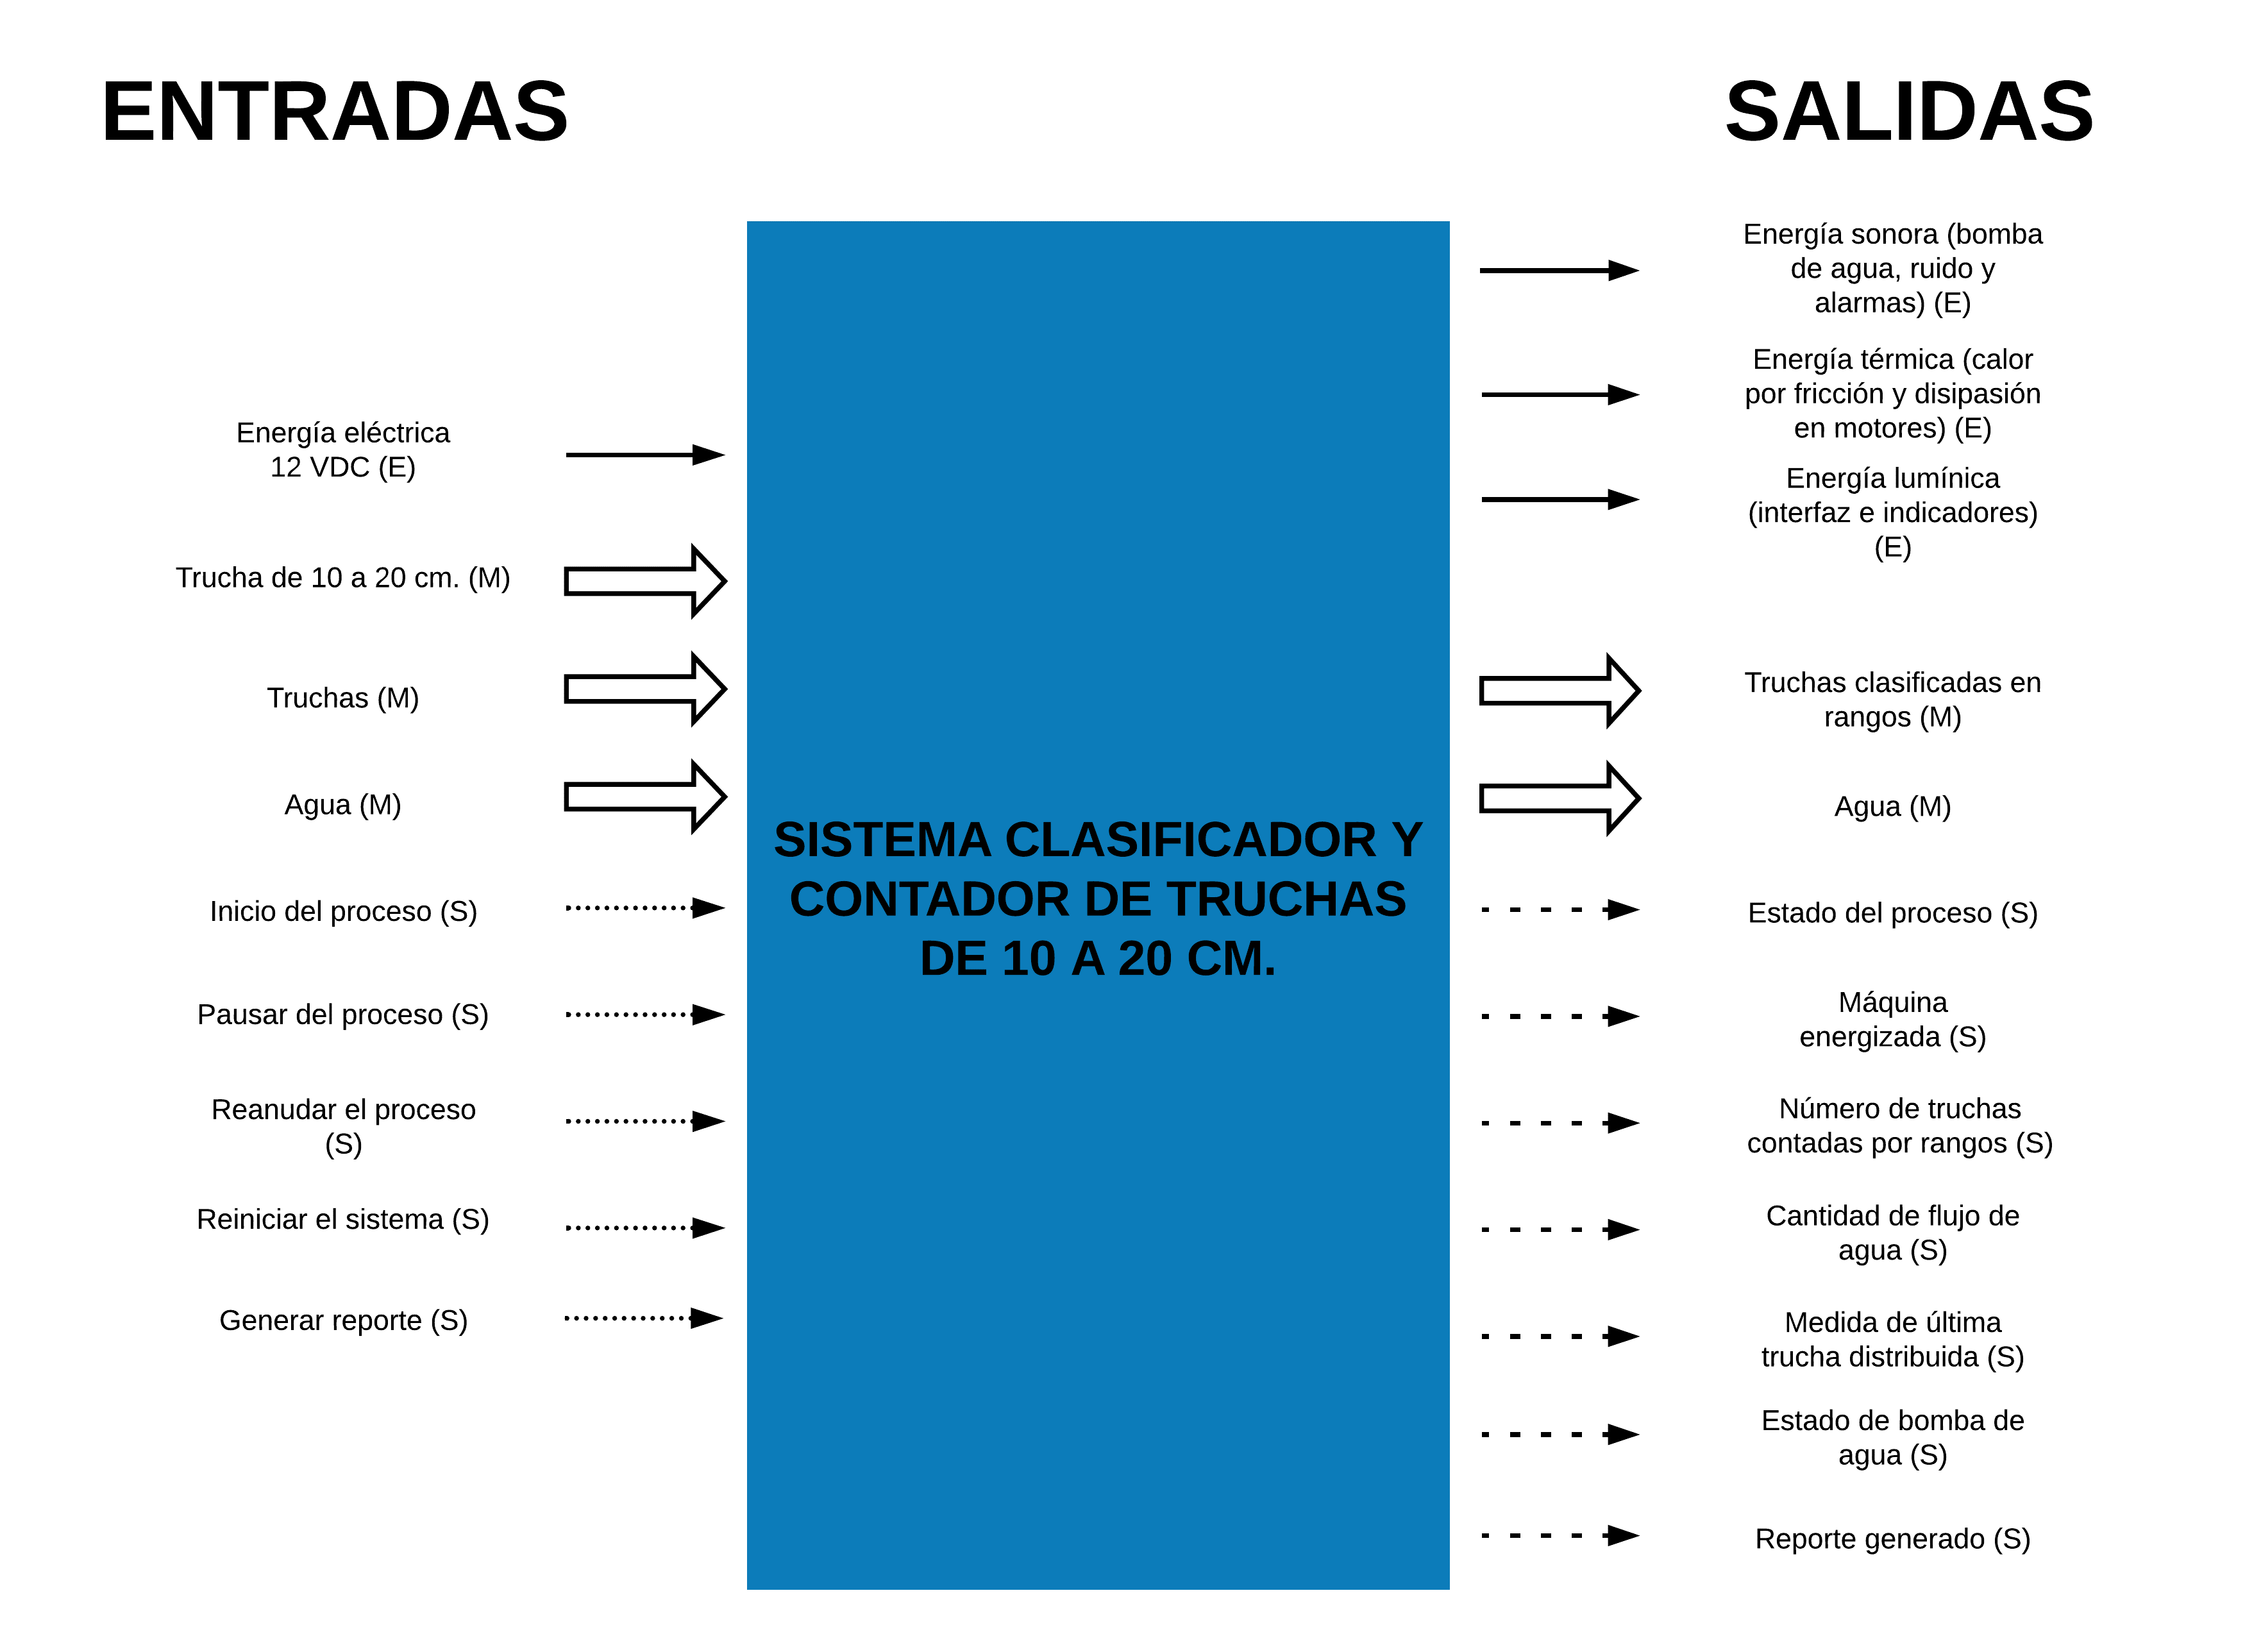
\includegraphics[width=1\textwidth]{chapter3/caja negra del sistema.png}
	\caption{Caja negra del sistema.}
	Fuente: Elaboración propia.
	\label{fig:caja negra del sistema}
\end{figure}

%% NUEVA SUB-SUB-SECCION X.X.X.X
\subsubsection{Función principal}

El sistema tiene como función principal clasificar truchas que provienen de un estanque o jaula flotante que tiene truchas que necesitan ser redistribuidas según sus dimensiones.

%% NUEVA SUB-SUB-SECCION X.X.X.X
\subsubsection{Entradas}

El sistema tiene entradas de diversos tipos: energía, materia y señal. La entrada de energía es únicamente una batería de 12 VDC ya que es portable; Las entradas de materia son indispensablemente el agua y las truchas a clasificar; Las señales de entrada para este proceso son las básicas para cualquier proceso de este tipo (\textit{iniciar, pausar, reanudar y reiniciar}), además la señal de generar un reporte para ser analizado y mantener control sobre el cultivo.

%% NUEVA SUB-SUB-SECCION X.X.X.X
\subsubsection{Salidas}

De manera similar a las entradas, las salidas se dividen en energía, materia y señal: El sistema genera tres tipos de energía debido a los actuadores, ruido, alarmas, interfaz e indicadores; Las truchas divididas en hasta tres rangos salen de manera separada; Se muestra el estado del proceso, estado del sistema, número de truchas contadas dependiendo del rango, medida de la última trucha distribuida, estado de la bomba de agua y la señal de reporte generado.

%% NUEVO SUBSECCION X.X.X
\subsection{Estructura de funciones}

Una vez que se ha formulado la caja negra es posible indicar, con el uso de diagrama de bloques, expresar la relación entre entradas y salidas con una solución neutral. Esta relación debe tener la mayor precisión posible. La estructura de funciones global puede desglosarse en sistemas que a su vez se subdividen en funciones.\cite[p.~169-181]{Pahl2007}

\newpage
\thispagestyle{mylandscape}
\begin{landscape}
	\begin{figure}[H]
		\centering
		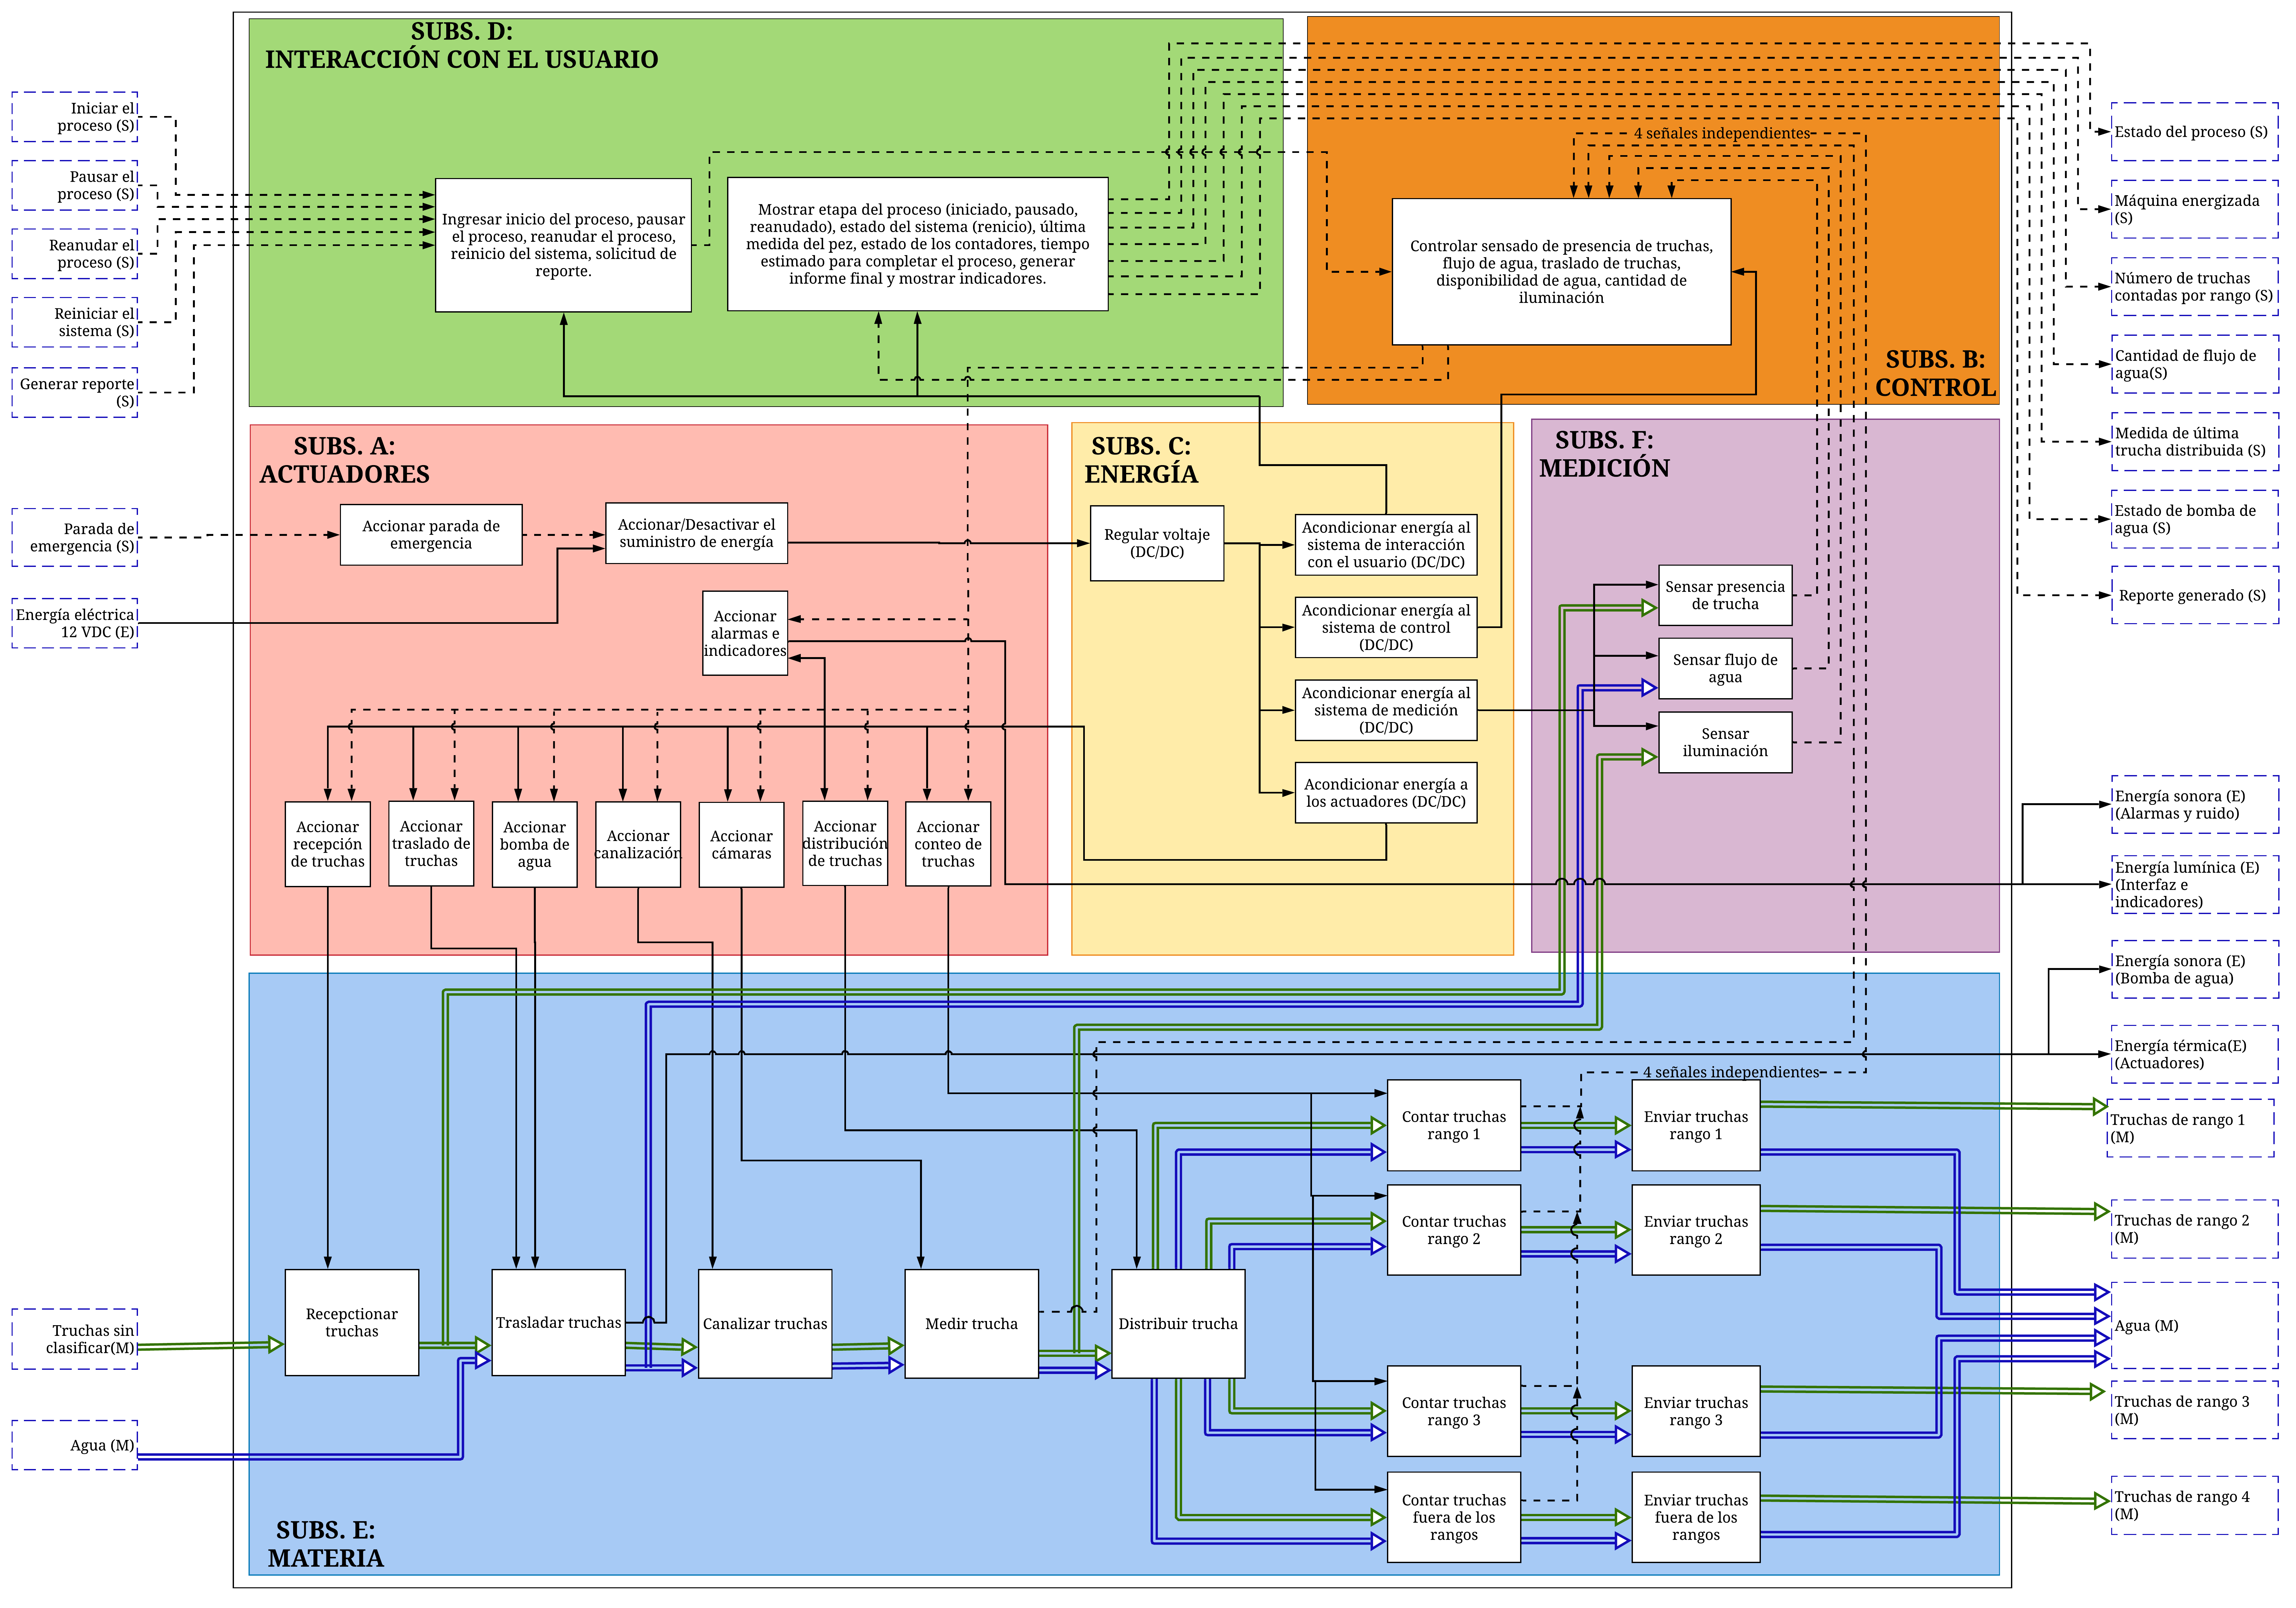
\includegraphics[width=0.98\paperwidth]{chapter3/estructura global de funciones.png}
		\caption{Estructura global de funciones.}
		Fuente: Elaboración propia.
		\label{fig:estructura global de funciones}
	\end{figure}
\end{landscape}


\newpage
\thispagestyle{fancy}
%% NUEVA SUB-SUB-SECCION X.X.X.X
\subsubsection{Lista de funciones por subsistema}

El sistema propuesto consta de seis subsistemas: actuadores, control, energía, interacción con el usuario, materia y medición. El propósito y funciones de cada subsistema se indica en las siguientes líneas.

\begin{enumerate}
	
	\item \textbf{Subsistema A: Actuadores}\\ El subsistema integra el accionamiento de los mecanismos que transforman que permiten distribuir la materia en los rangos requeridos.
	
	\begin{enumerate}[label=\Alph*)] % \alph for lowercase
		\item	\textbf{Accionar parada de emergencia:} Esta función permite conectar o desconectar físicamente la energía de en-trada del resto del sistema.
		
		\item	\textbf{Accionar/Desactivar el suministro de energía:} Esta función se encargará de proveer energía al sistema para dar inicio al proceso al momento que recibe la señal de inicio.
		
		\item	\textbf{Accionar recepción de truchas:} Esta función activa o desactiva la entrada de materia al sistema, en este caso el ingreso de truchas al sistema.
		
		\item	\textbf{Accionar traslado de truchas:} Esta función activa o desactiva la función que recibe truchas y agua para poder desplazar a las truchas dentro del sistema.
		
		\item	\textbf{Accionar bomba de agua:} Esta función activa, desactiva y regula el flujo de agua dentro del sistema. 
		
		\item	\textbf{Accionar iluminación:} Esta función activa o desactiva la iluminación necesaria para las cámaras.			
		
		\item	\textbf{Accionar cámaras:} Esta función activa, desactiva y prepara la adquisición de imágenes o video del sistema.
		
		\item	\textbf{Accionar distribución de truchas:} Esta función se encarga de la distribución de las truchas según su rango dentro del sistema.
		
		\item	\textbf{Accionar alarmas e indicadores:} Acciona las alarmas e indicadores del sistema para poder informar al operario de la situación del proceso.
		
	\end{enumerate}
	
	\item \textbf{Subsistema B: Control}\\ El subsistema de control garantiza la precisión de los mecanismos, la calidad de los procesos, la seguridad del sistema.
	\begin{enumerate}[label=\Alph*)] % \alph for lowercase
		\item \textbf{Función general:} Esta función controla el sensado de presencia de trucha, flujo de agua, traslado de truchas, sensado de disponibilidad de agua y cantidad de iluminación.			
	\end{enumerate}
	
	\item \textbf{Subsistema C: Energía}\\ El subsistema de energía mantiene el funcionamiento continuo del sistema para reali-zar sus funciones características a través de una fuente de energía. 
	
	\begin{enumerate}[label=\Alph*)] % \alph for lowercase
		\item	\textbf{Regular voltaje ($ DC/DC $):} Esta función acondiciona la energía de entrada (12 VDC) a la energía necesaria para el sistema.
		
		\item	\textbf{Acondicionar energía al sistema de interacción con el usuario ($ DC/DC $):}		Esta función acondiciona la energía de entrada (12 VDC) a la energía necesaria para el sistema de interacción con el usuario.
		
		\item	\textbf{Acondicionar energía al sistema de control ($ DC/DC $):} Esta función acondiciona la energía de entrada (12 VDC) a la energía necesaria para el sistema de control
		
		\item	\textbf{Acondicionar energía al sistema de medición ($ DC/DC $):} Esta función acondiciona la energía de entrada (12 VDC) a la energía necesaria para el sistema de medición.
		
		\item	\textbf{Acondicionar energía a los actuadores ($ DC/DC $):} Esta función acondiciona la energía de entrada (12 VDC) a la energía necesaria para el sistema de los actuadores.
		
	\end{enumerate}
	
	\item \textbf{Subsistema D: Interacción con el usuario}\\ Este subsistema permite la comunicación entre el usuario final / operador y el sistema. Facilita la realización del proceso completo, permitiendo al usuario contar con información importante del proceso para poder tomar decisiones de forma rápida.
	
	\begin{enumerate}[label=\Alph*)] % \alph for lowercase
		\item	\textbf{Función ingreso de señales:} Esta función recibe las señales de entrada como \textit{inicio, pausar, reanudar y reiniciar} el proceso. Además, recibe la solicitud de reporte. Usa esta información y la envía al subsistema de control.
		
		\item	\textbf{Función mostrar señales:} Esta función muestra las etapas del proceso (\textit{iniciar, pausar, reanudar y reiniciar}). También muestra la medida de la última trucha que se distribuyó, estado de los contadores, tiempo estimado para completar el proceso, informe generado y mostrar indicadores.
		
	\end{enumerate}
	
	\item \textbf{Subsistema E: Materia}\\ El subsistema de materia contiene las funciones que se encargan de distribuir la mate-ria en rangos que se ingresan al sistema. Las funciones se desarrollan como una secuencia de tareas.
	
	\begin{enumerate}[label=\Alph*)] % \alph for lowercase
		
		\item	\textbf{Recepcionar truchas:} Esta función mediante mecanismos recibe indicaciones de otras partes del sistema para accionarse. Es el primer módulo que recepciona a las truchas. 
		
		\item	\textbf{Trasladar truchas:} Este mecanismo recibe agua y a las truchas que salen de la función "\textit{recepcionar truchas}". Impulsa mediante un flujo de agua constante a las truchas a lo largo del sistema hasta llegar a las salidas.
		
		\item	\textbf{Canalizar truchas:} Este mecanismo recibe agua y truchas del módulo "\textit{trasladar truchas}". Además, es accionado por actuadores para cumplir con dejar pasar una trucha por vez al siguiente módulo del sistema.
		
		\item	\textbf{Medir y contar trucha:} Esta función ejecuta algoritmos para poder medir y contar una trucha, además decide qué camino tomará la trucha en el mecanismo de "\textit{distribuir trucha}". Este mecanismo recibe señales de control y envía información sobre las dimensiones y conteo de las truchas al sistema de control.
		
		\item	\textbf{Distribuir trucha:} Este mecanismo recibe agua y trucha medida del módulo anterior "\textit{medir trucha}". Es accionada y permite seleccionar según los rangos el próximo módulo correspondiente. Este módulo es el encargado de clasificar físicamente a la trucha.
		
	\end{enumerate}
	
	
	\item \textbf{Subsistema F: Medición}\\ El subsistema de medición se encarga de sensar las variables del proceso necesarias para ejercer un óptimo control del sistema y minimizar el error. Se considera las siguientes funciones como esenciales.
	
	\begin{enumerate}[label=\Alph*)] % \alph for lowercase
		\item	\textbf{Sensar presencia de trucha:} Esta función detecta si las truchas han ingresado al sistema o siguen dentro del sistema.
		
		\item	\textbf{Sensar flujo de agua:} Esta función mide el flujo de agua dentro del sistema para mantenerlo constante para reducir el estrés hídrico.
		
		\item	\textbf{Sensar iluminación:} Esta función sensa la iluminación que es necesaria para capturar imágenes con normalidad.
		
	\end{enumerate}	
	
	
	
	%	To create new enumerate alpha use code below
	%	\begin{enumerate}[label=\Alph*)] % \alph for lowercase
	%	\end{enumerate}
\end{enumerate}
%% NUEVO SUBSECCION X.X.X
\subsection{Matriz morfológica}

La matriz morfológica brinda posibles soluciones a los propósitos de cada función. Cada solución posee un principio de funcionamiento diferente. La búsqueda de posibles soluciones se basa en analizar las entradas/salidas de señales, energía y materia de cada función y proponer un dispositivo, mecanismo o sistema que pueda satisfacer la tarea.\cite[p.~181-184]{Pahl2007}

\newpage
\pagestyle{mylandscape}

\begin{landscape}
	% Please add the following required packages to your document preamble:
	% \usepackage[table,xcdraw]{xcolor}
	% If you use beamer only pass "xcolor=table" option, i.e. \documentclass[xcolor=table]{beamer}
	% \usepackage{longtable}
	% Note: It may be necessary to compile the document several times to get a multi-page table to line up properly
	% Please add the following required packages to your document preamble:
	% \usepackage[table,xcdraw]{xcolor}
	% If you use beamer only pass "xcolor=table" option, i.e. \documentclass[xcolor=table]{beamer}
	% \usepackage{longtable}
	% Note: It may be necessary to compile the document several times to get a multi-page table to line up properly
	% Please add the following required packages to your document preamble:
	% \usepackage[table,xcdraw]{xcolor}
	% If you use beamer only pass "xcolor=table" option, i.e. \documentclass[xcolor=table]{beamer}
	% \usepackage{longtable}
	% Note: It may be necessary to compile the document several times to get a multi-page table to line up properly
	\begin{longtable}{|
			>{\columncolor[HTML]{D9D9D9}}c |c|l|l|c|l|c|c|l|c|c|c|l|c|l|l|}
		\caption{Matriz morfológica del subsistema A}
		\label{tab:matriz morfologica del subsistema a}\\
		\hline
		\cellcolor[HTML]{A6A6A6}{\color[HTML]{000000} \textbf{Función}} &
		\multicolumn{15}{c|}{\cellcolor[HTML]{A6A6A6}{\color[HTML]{000000} \textbf{Posibles soluciones}}} \\ \hline
		\endfirsthead
		%
		\multicolumn{16}{c}%
		{{Tabla \thetable\ continuación de la página anterior.}} \\
		\hline
		\cellcolor[HTML]{A6A6A6}{\color[HTML]{000000} \textbf{Función}} &
		\multicolumn{15}{c|}{\cellcolor[HTML]{A6A6A6}{\color[HTML]{000000} \textbf{Posibles soluciones}}} \\ \hline
		\endhead
		%
		\cellcolor[HTML]{D9D9D9}{\color[HTML]{000000} \begin{tabular}[c]{@{}c@{}}Accionar \\ parada de emergencia\end{tabular}} &
		\multicolumn{5}{c|}{			
			\begin{minipage}{0.20\textwidth}
				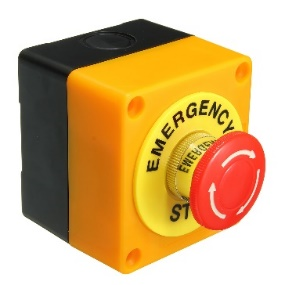
\includegraphics[width=1\textwidth]{chapter3/matriz/boton de emergencia.png}
				\\ Botón de emergencia.
		\end{minipage}} &
		\multicolumn{5}{c|}{Interruptor de emergencia} &
		\multicolumn{5}{c|}{\begin{tabular}[c]{@{}c@{}}Interruptor de doble estado\\ de apagado de emergencia\end{tabular}} \\ \hline
		\cellcolor[HTML]{D9D9D9}{\color[HTML]{000000} \begin{tabular}[c]{@{}c@{}}Accionar/Desactivar\\ el suministro de energía\end{tabular}} &
		\multicolumn{3}{c|}{Switch} &
		\multicolumn{3}{c|}{Interruptor tipo botón} &
		\multicolumn{3}{c|}{Actuador de cabeza de palanca} &
		\multicolumn{3}{c|}{Interruptor de palanca} &
		\multicolumn{3}{c|}{Interruptor deslizante} \\ \hline
		\cellcolor[HTML]{D9D9D9}{\color[HTML]{000000} \begin{tabular}[c]{@{}c@{}}Accionar\\ recepción de truchas\end{tabular}} &
		\multicolumn{5}{c|}{Vávula accionada por servomotor} &
		\multicolumn{5}{c|}{Válvula de compuertas} &
		\multicolumn{5}{c|}{Reja accionada por motor} \\ \hline
		\cellcolor[HTML]{D9D9D9}{\color[HTML]{000000} \begin{tabular}[c]{@{}c@{}}Accionar\\ traslado de truchas\end{tabular}} &
		\multicolumn{5}{c|}{Electroválvula solenoide} &
		\multicolumn{5}{c|}{Electroválvula de acción indirecta} &
		\multicolumn{5}{c|}{Electroválvula de acción mixta} \\ \hline
		\begin{tabular}[c]{@{}c@{}}Accionar\\ bomba de agua\end{tabular} &
		\multicolumn{3}{c|}{\begin{tabular}[c]{@{}c@{}}Bomba de agua\\ centrífuga\end{tabular}} &
		\multicolumn{3}{c|}{\begin{tabular}[c]{@{}c@{}}Bomba de agua\\ sumergible\end{tabular}} &
		\multicolumn{3}{c|}{Bomba de refuerzo} &
		\multicolumn{3}{c|}{Electrobomba} &
		\multicolumn{3}{c|}{Motobomba} \\ \hline
		\begin{tabular}[c]{@{}c@{}}Accionar\\ iluminación\end{tabular} &
		\multicolumn{8}{c|}{Led de alta potencia} &
		\multicolumn{7}{c|}{LED reflector} \\ \hline
		\begin{tabular}[c]{@{}c@{}}Accionar\\ cámaras\end{tabular} &
		\multicolumn{5}{c|}{Módulo con cámara} &
		\multicolumn{5}{c|}{Cámara estéreo} &
		\multicolumn{5}{c|}{Cámara infrarroja} \\ \hline
		\begin{tabular}[c]{@{}c@{}}Accionar\\ distribución de truchas\end{tabular} &
		\multicolumn{8}{c|}{Sevomotor} &
		\multicolumn{7}{c|}{Actuador eléctrico} \\ \hline
		\begin{tabular}[c]{@{}c@{}}Accionar \\ alarmas e indicadores\end{tabular} &
		\multicolumn{5}{c|}{Timbre} &
		\multicolumn{5}{c|}{Bocina} &
		\multicolumn{5}{c|}{Indicadora visual} \\ \hline
	\end{longtable}
	\begin{center}
		Fuente: Geekboleteletronics Hawkusa, Homedepot, Parts-express, TcPoolEquipment, Uctronics, Eco-sources, imágenes de dominio público y elaboración propia.
	\end{center}
	
	%%%%%%%%%%%%%%%%%%%%%%%%%%%%%%%%%%%%%%%%%%%%%%%%%%%%%%%%%%%%%%%%%%%%%%%%%%%%%%%%%%%%%%%%%%%%%%%%%%%%
	
	% Please add the following required packages to your document preamble:
	% \usepackage[table,xcdraw]{xcolor}
	% If you use beamer only pass "xcolor=table" option, i.e. \documentclass[xcolor=table]{beamer}
	% \usepackage{longtable}
	% Note: It may be necessary to compile the document several times to get a multi-page table to line up properly
	\begin{longtable}{|
			>{\columncolor[HTML]{A6A6A6}}c |c|c|c|c|}
		\caption{Matriz morfolófica del subsistema B}
		\label{tab:matriz morfológica del sistema b}\\
		\hline
		{\color[HTML]{000000} \textbf{Función}} &
		\multicolumn{4}{c|}{\cellcolor[HTML]{A6A6A6}{\color[HTML]{000000} \textbf{Posibles soluciones}}} \\ \hline
		\endfirsthead
		%
		\multicolumn{5}{c}%
		{{Tabla \thetable\ continuación de la página anterior.}} \\
		\hline
		{\color[HTML]{000000} \textbf{Función}} &
		\multicolumn{4}{c|}{\cellcolor[HTML]{A6A6A6}{\color[HTML]{000000} \textbf{Posibles soluciones}}} \\ \hline
		\endhead
		%
		\cellcolor[HTML]{D9D9D9}{\color[HTML]{000000} \begin{tabular}[c]{@{}c@{}}Función general: sensado de \\ presencia de trucha, flujo de\\  agua, traslado de truchas, \\ sensado de disponibilidad \\ de agua y cantidad de \\ iluminación.\end{tabular}} &
		Microcontrolador &
		\begin{tabular}[c]{@{}c@{}}Controlador lógico\\ programable\end{tabular} &
		\begin{tabular}[c]{@{}c@{}}Computadora\\ monoplaca\end{tabular} &
		Computadora ordinaria \\ \hline
	\end{longtable}
	\begin{center}
		Fuente: Imágenes de dominio público y elaboración propia.
	\end{center}
	
	
	% Please add the following required packages to your document preamble:
	% \usepackage{multirow}
	% \usepackage[table,xcdraw]{xcolor}
	% If you use beamer only pass "xcolor=table" option, i.e. \documentclass[xcolor=table]{beamer}
	% \usepackage{longtable}
	% Note: It may be necessary to compile the document several times to get a multi-page table to line up properly
	\begin{longtable}{|
			>{\columncolor[HTML]{D9D9D9}}c |c|c|}
		\caption{Matriz morfológica subsistema C}
		\label{tab:matriz morfologica subsistema c}\\
		\hline
		\cellcolor[HTML]{A6A6A6}{\color[HTML]{000000} \textbf{Función}} &
		\multicolumn{2}{c|}{\cellcolor[HTML]{A6A6A6}{\color[HTML]{000000} \textbf{Posibles soluciones}}} \\ \hline
		\endfirsthead
		%
		\multicolumn{3}{c}%
		{{Tabla \thetable\ continuación de la página anterior.}} \\
		\hline
		\cellcolor[HTML]{A6A6A6}{\color[HTML]{000000} \textbf{Función}} &
		\multicolumn{2}{c|}{\cellcolor[HTML]{A6A6A6}{\color[HTML]{000000} \textbf{Posibles soluciones}}} \\ \hline
		\endhead
		%
		{\color[HTML]{000000} Acondicionar voltaje (AC/DC)}                                                             & \multicolumn{2}{c|}{Fuente de alimentación} \\ \hline
		Regular voltaje (DC/DC)                                                                                         &                      &                      \\ \cline{1-1}
		\begin{tabular}[c]{@{}c@{}}Acondicionar energía al sistema de\\ interacción con el usuario (DC/DC)\end{tabular} &                      &                      \\ \cline{1-1}
		\begin{tabular}[c]{@{}c@{}}Acondicionar energía al sistema de\\ control (DC/DC)\end{tabular} &
		&
		\multirow{-3}{*}{Variador de voltaje} \\ \cline{1-1} \cline{3-3} 
		\begin{tabular}[c]{@{}c@{}}Acondicionar energía al sistema de\\ medición (DC/DC)\end{tabular}                   &                      &                      \\ \cline{1-1}
		\begin{tabular}[c]{@{}c@{}}Acondicionar energía a los \\ actuadores (DC/DC)\end{tabular} &
		\multirow{-5}{*}{Transformador rectificador} &
		\multirow{-2}{*}{Fuente switching} \\ \hline
	\end{longtable}
	
	\begin{center}
		Fuente: Imágenes de dominio público y elaboración propia.
	\end{center}
	
	
	% Please add the following required packages to your document preamble:
	% \usepackage{multirow}
	% \usepackage[table,xcdraw]{xcolor}
	% If you use beamer only pass "xcolor=table" option, i.e. \documentclass[xcolor=table]{beamer}
	% \usepackage{longtable}
	% Note: It may be necessary to compile the document several times to get a multi-page table to line up properly
	\begin{longtable}{|
			>{\columncolor[HTML]{D9D9D9}}c |c|c|l|}
		\caption{Matriz morfológica del subsistema D.}
		\label{tab:matriz morfologica del subsistema d}\\
		\hline
		\cellcolor[HTML]{A6A6A6}{\color[HTML]{000000} \textbf{Función}} &
		\multicolumn{3}{c|}{\cellcolor[HTML]{A6A6A6}{\color[HTML]{000000} \textbf{Posibles soluciones}}} \\ \hline
		\endfirsthead
		%
		\multicolumn{4}{c}%
		{{Tabla \thetable\ continuación de la página anterior.}} \\
		\hline
		\cellcolor[HTML]{A6A6A6}{\color[HTML]{000000} \textbf{Función}} &
		\multicolumn{3}{c|}{\cellcolor[HTML]{A6A6A6}{\color[HTML]{000000} \textbf{Posibles soluciones}}} \\ \hline
		\endhead
		%
		\begin{tabular}[c]{@{}c@{}}Función ingreso de señales:\\ iniciar, pausar, reanudar y \\ reiniciar el proces\end{tabular} &
		&
		&
		\\ \cline{1-1}
		\begin{tabular}[c]{@{}c@{}}Función mostrar señales:\\ iniciar, pausar, reanudar y\\ reiniciar el proceso\end{tabular} &
		\multirow{-2}{*}{Aplicación en celular} &
		\multirow{-2}{*}{Interfaz con el usuario en computadora} &
		\multirow{-2}{*}{Panel de control con botones e indicadores} \\ \hline
	\end{longtable}
	
	\begin{center}
		Fuente: Imágenes de dominio público y elaboración propia.
	\end{center}
	
	% Please add the following required packages to your document preamble:
	% \usepackage[table,xcdraw]{xcolor}
	% If you use beamer only pass "xcolor=table" option, i.e. \documentclass[xcolor=table]{beamer}
	% \usepackage{longtable}
	% Note: It may be necessary to compile the document several times to get a multi-page table to line up properly
	\begin{longtable}{|
			>{\columncolor[HTML]{D9D9D9}}c |c|l|c|c|c|l|}
		\caption{Matriz morfológica del subsistema E.}
		\label{tab:matriz morfologica del subsistema e}\\
		\hline
		\cellcolor[HTML]{A6A6A6}{\color[HTML]{000000} \textbf{Función}} &
		\multicolumn{6}{c|}{\cellcolor[HTML]{A6A6A6}{\color[HTML]{000000} \textbf{Posibles soluciones}}} \\ \hline
		\endfirsthead
		%
		\multicolumn{7}{c}%
		{{Tabla \thetable\ continuación de la página anterior.}} \\
		\hline
		\cellcolor[HTML]{A6A6A6}{\color[HTML]{000000} \textbf{Función}} &
		\multicolumn{6}{c|}{\cellcolor[HTML]{A6A6A6}{\color[HTML]{000000} \textbf{Posibles soluciones}}} \\ \hline
		\endhead
		%
		Recepcionar truchas & \multicolumn{3}{c|}{Tolva}                     & \multicolumn{3}{c|}{Malla}                             \\ \hline
		Trasladar truchas &
		\multicolumn{2}{c|}{Inyección de caudal} &
		\multicolumn{2}{c|}{Juego de pistones} &
		\multicolumn{2}{c|}{Cadenas transportadoras} \\ \hline
		Canalizar truhas    & \multicolumn{2}{c|}{Tolva} & \multicolumn{2}{c|}{Filtros de tamaño} & \multicolumn{2}{c|}{Filtro único} \\ \hline
		Distribuir truchas &
		\multicolumn{2}{c|}{Múltiples compuertas programables} &
		\multicolumn{2}{c|}{Compuerta única programable} &
		\multicolumn{2}{c|}{Dimensionalidad} \\ \hline
	\end{longtable}
	
	\begin{center}
		Fuente: FAO, imágenes de dominio público y elaboración propia.
	\end{center}
	
	
	% Please add the following required packages to your document preamble:
	% \usepackage[table,xcdraw]{xcolor}
	% If you use beamer only pass "xcolor=table" option, i.e. \documentclass[xcolor=table]{beamer}
	% \usepackage{longtable}
	% Note: It may be necessary to compile the document several times to get a multi-page table to line up properly
	\begin{longtable}{|
			>{\columncolor[HTML]{D9D9D9}}c |c|c|c|c|c|}
		\caption{Matriz morfológica del subsistema F}
		\label{tab:matriz morfológica del subsistema f}\\
		\hline
		\cellcolor[HTML]{A6A6A6}{\color[HTML]{000000} \textbf{Función}} &
		\multicolumn{5}{c|}{\cellcolor[HTML]{A6A6A6}{\color[HTML]{000000} \textbf{Posibles soluciones}}} \\ \hline
		\endfirsthead
		%
		\multicolumn{6}{c}%
		{{Tabla \thetable\ continuación de la página anterior.}} \\
		\hline
		\cellcolor[HTML]{A6A6A6}{\color[HTML]{000000} \textbf{Función}} &
		\multicolumn{5}{c|}{\cellcolor[HTML]{A6A6A6}{\color[HTML]{000000} \textbf{Posibles soluciones}}} \\ \hline
		\endhead
		%
		\begin{tabular}[c]{@{}c@{}}Sensar presencia\\ de trucha\end{tabular} &
		Sensor de presencia &
		Fotorresistencia y láser &
		Sensor infrarrojo &
		Sensor de ultrasonido &
		Sensor de peso \\ \hline
		\begin{tabular}[c]{@{}c@{}}Sensar\\ flujo de agua\end{tabular} &
		Sensor de caudal &
		Rotámetro electrónico &
		\begin{tabular}[c]{@{}c@{}}Tubos de Venturi y\\ sensores de presión\end{tabular} &
		\begin{tabular}[c]{@{}c@{}}Medidor de flujo\\ de velocidad\end{tabular} &
		\begin{tabular}[c]{@{}c@{}}Sensor de presión \\ líquida\end{tabular} \\ \hline
		\begin{tabular}[c]{@{}c@{}}Sensar\\ iluminación\end{tabular} &
		\multicolumn{5}{c|}{Sensor electrónico} \\ \hline
	\end{longtable}
	
	\begin{center}
		Fuente: Teslabem, Bigtronica, Arduino e imágenes de dominio público.
	\end{center}
	
\end{landscape}


\newpage
\pagestyle{myportland}

%% NUEVO SUBSECCION X.X.X
\subsection{Conceptos de solución}

Los conceptos de solución que se presentan a continuación deben dar solución acorde a la problemática. En la Figura \ref{fig:dibujo conceptual de la problematica} se muestra un dibujo de dicha problemática.

\begin{figure}[H]
	\centering
	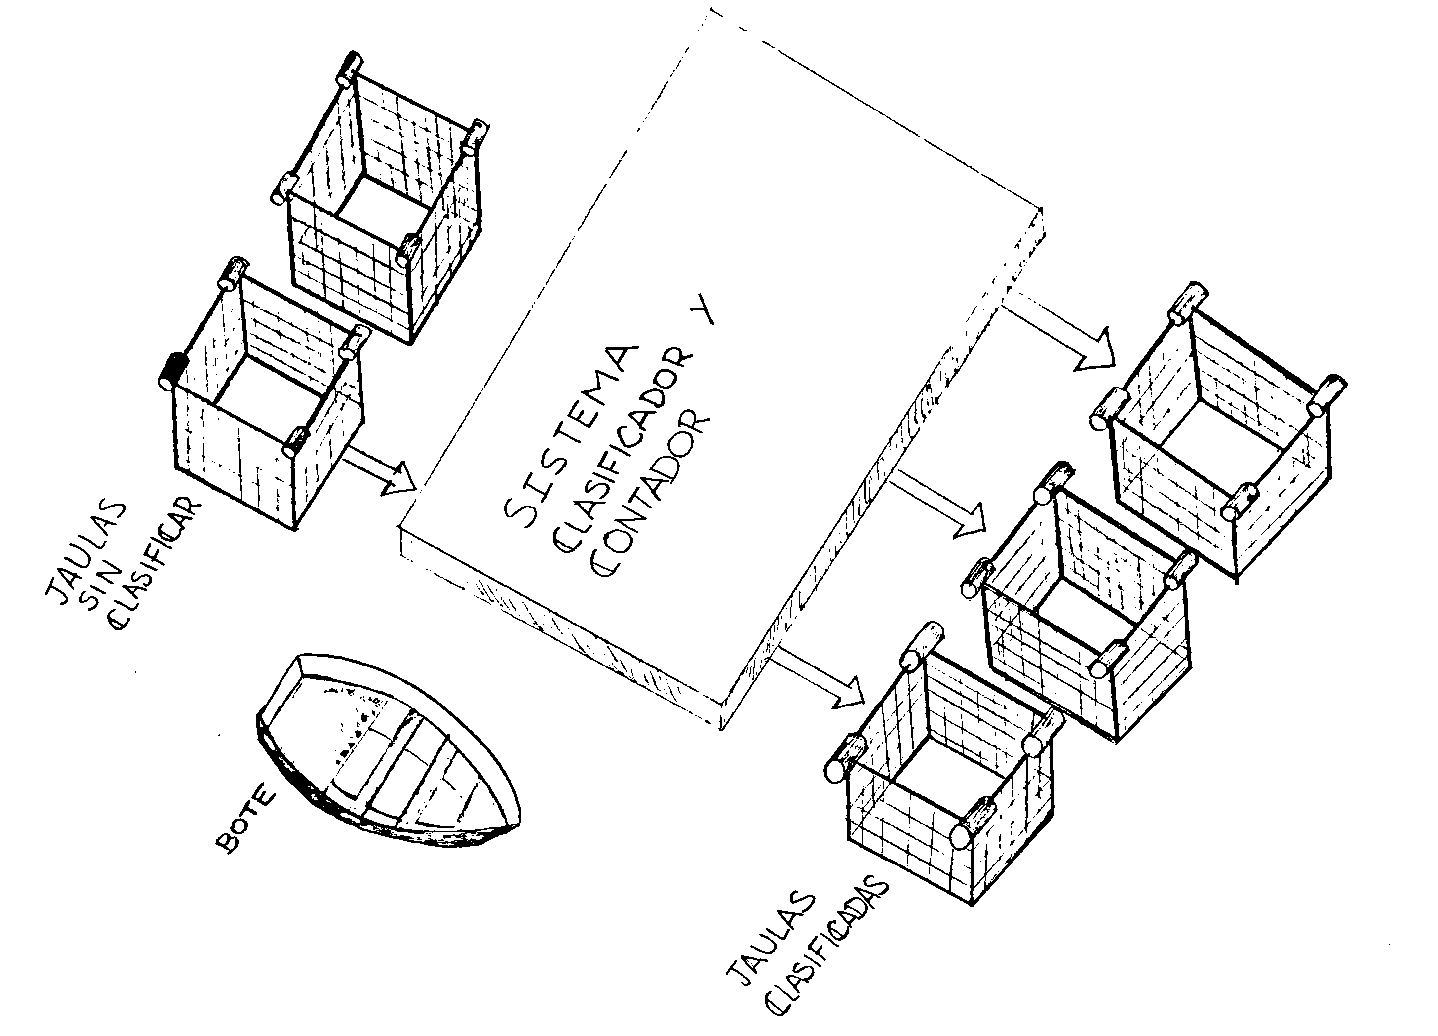
\includegraphics[width=1\textwidth]{chapter3/dibujo conceptual de la problematica.png}
	\caption{Dibujo conceptual de la problemática.}
	Fuente: Elaboración propia.
	\label{fig:dibujo conceptual de la problematica}
\end{figure}

%% NUEVA SUB-SUB-SECCION X.X.X.X
\subsubsection{Concepto de solución N° 1}

El sistema (Figura \ref{fig:dibujo de concepto de solucion 1}) hace uso de una plataforma flotante y una mesa como soporte para el sistema. En el dibujo se ha omitido los cilindros que mantienen a flote la plataforma. El sistema cuenta con cuatro sistemas físicos separados que son acoplados en la parte central de la mesa. Para iniciar el funcionamiento el operario debe verificar que el interruptor de seguridad se encuentra des-activado. Luego de verificar debe accionar mediante el uso de un switch la energización del sistema y con esto accionar a su vez el flujo de agua debido a la activación de la bomba sumergible.

Una vez realizada la preparación del sistema la reja accionada mediante un motor que acciona el sistema piñón-cremallera debe dejar el paso de truchas al siguiente sistema físico. El operario debe extraer mediante una sacadera truchas de la jaula sin clasificar y depositarlas en el sistema físico de recepción. Las truchas avanzarán debido al flujo de agua constante y la gravedad. A continuación, las truchas pasan por un filtro de tamaño para evitar la conglomeración. En el siguiente sistema físico las truchas son medidas y contadas mediante el uso de cámaras, que a su vez usan sistemas de iluminación. Con la información adquirida, el sistema decide el direccionamiento de compuertas para que la trucha pueda salir por el canal adecuado, con el uso de cámaras verifica su correcto funcionamiento.
El sistema puede ser desensamblado ya que se instala en una mesa hueca en el centro que permite el posicionamiento de esta, brindando así la posibilidad de cambios a cualquiera de las cuatro partes físicas.


\begin{figure}[H]
	\centering
	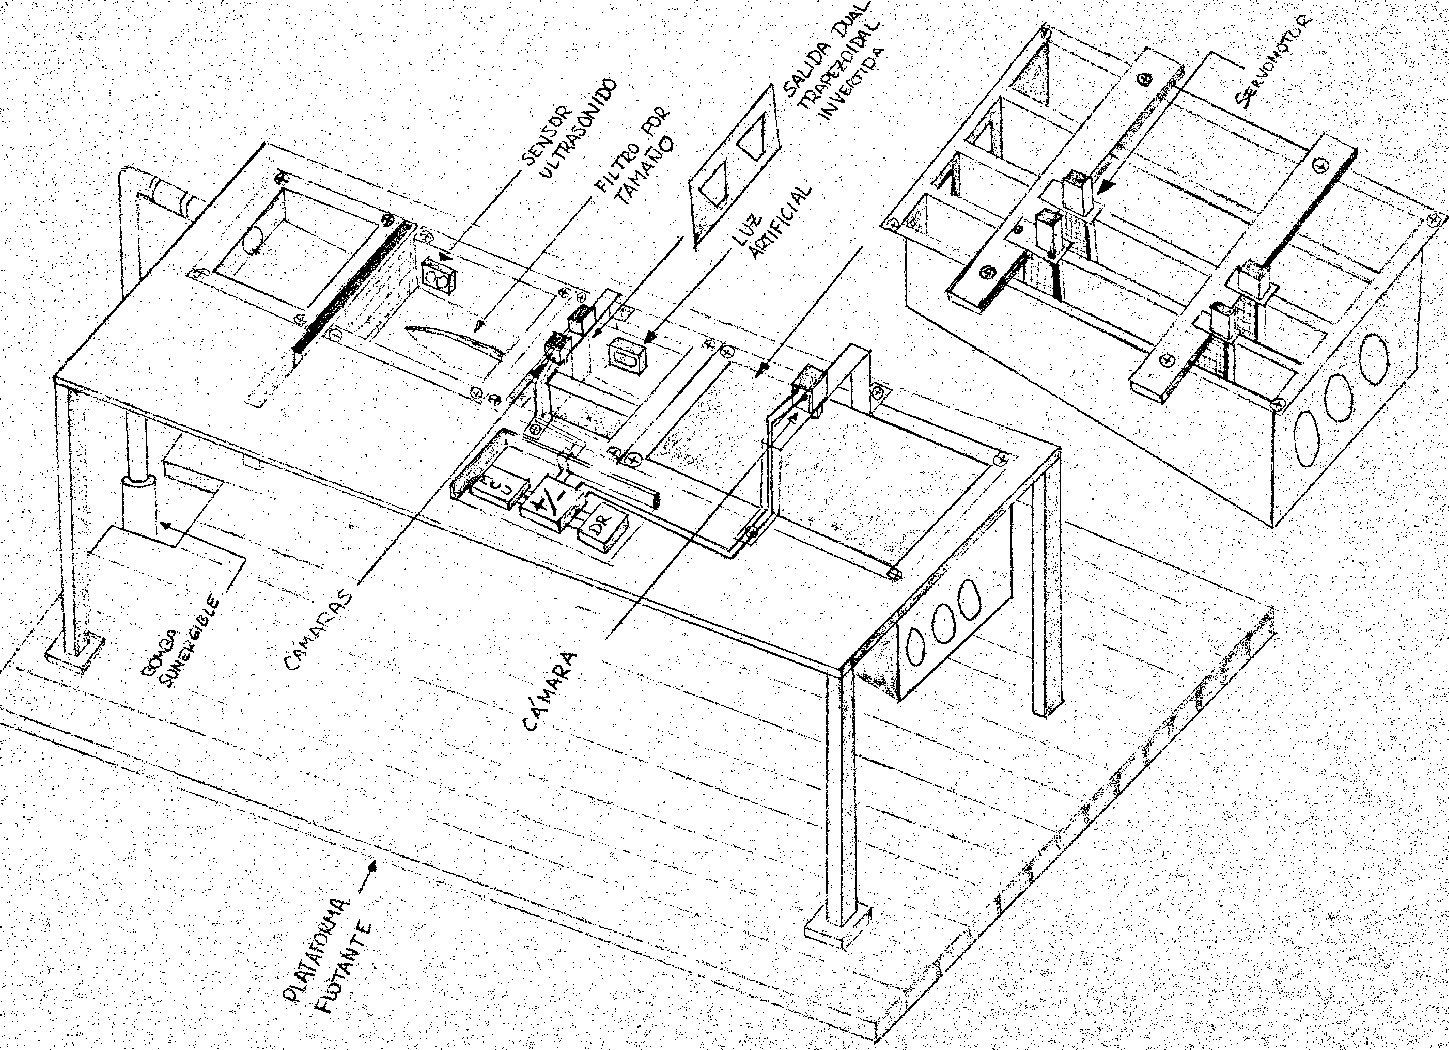
\includegraphics[width=0.85\textwidth]{chapter3/dibujo de concepto de solucion 1.png}
	\caption{Dibujo de concepto de solución N° 1.}
	Fuente: Elaboración propia.
	\label{fig:dibujo de concepto de solucion 1}
\end{figure}


%% NUEVA SUB-SUB-SECCION X.X.X.X
\subsubsection{Concepto de solución N° 2}

El sistema (Figura \ref{fig:dibujo de concepto de solucion 2}) cuenta con cuatro secciones físicas: "recepción y traslado de peces", "canalización, medición y conteo", "distribución" y "control". Estas secciones físicas están unidas con tubos plásticos transparentes y cables. Antes de empezar a usar el sistema, se debe verificar si el botón de emergencia está activado, de forma similar el actuador tipo hongo para verificar si el siste-ma está en accionamiento. Luego de revisar, se acciona la bomba sumergible y se acciona la electro-válvula para agregar el flujo de agua que trasladará a las truchas y verificar así la existencia de fugas.

Terminada la preparación, un operario con una sacadera empieza extrayendo truchas de una jaula sin clasificar y depositando las truchas en el sistema físico de "recepción de truchas". Las truchas depositadas resbalan por la tolva y se trasladan hacia las tuberías de reducción que funcionan como "canalizadores" (evita conglomeración). Estas tuberías de diámetro distinto permiten la medición del caudal para su control mediante el principio de Venturi, en este caso con el uso de sensores de presión. Además, la "detección de presencia de truchas" se da también en este sistema físico mediante sensores infrarrojos. Luego, la trucha es medida y contada por una cámara estéreo que indica al sistema físico de distribución la tubería de salida que la trucha debe tomar. La "distribución de truchas" emplea servomotores que direccionan la salida a la trucha a una salida. Para evitar la presión del agua sobre las compuertas controladas por los servomotores se emplea una rejilla para que el agua pase por una sección inferior. 
Durante todo el proceso, el microcontrolador envía inalámbricamente a un teléfono inteligente datos sobre las dimensiones de la trucha y el conteo. Al finalizar el proceso, se muestra un resumen en el teléfono sobre la clasificación y conteo de truchas.

\begin{figure}[H]
	\centering
	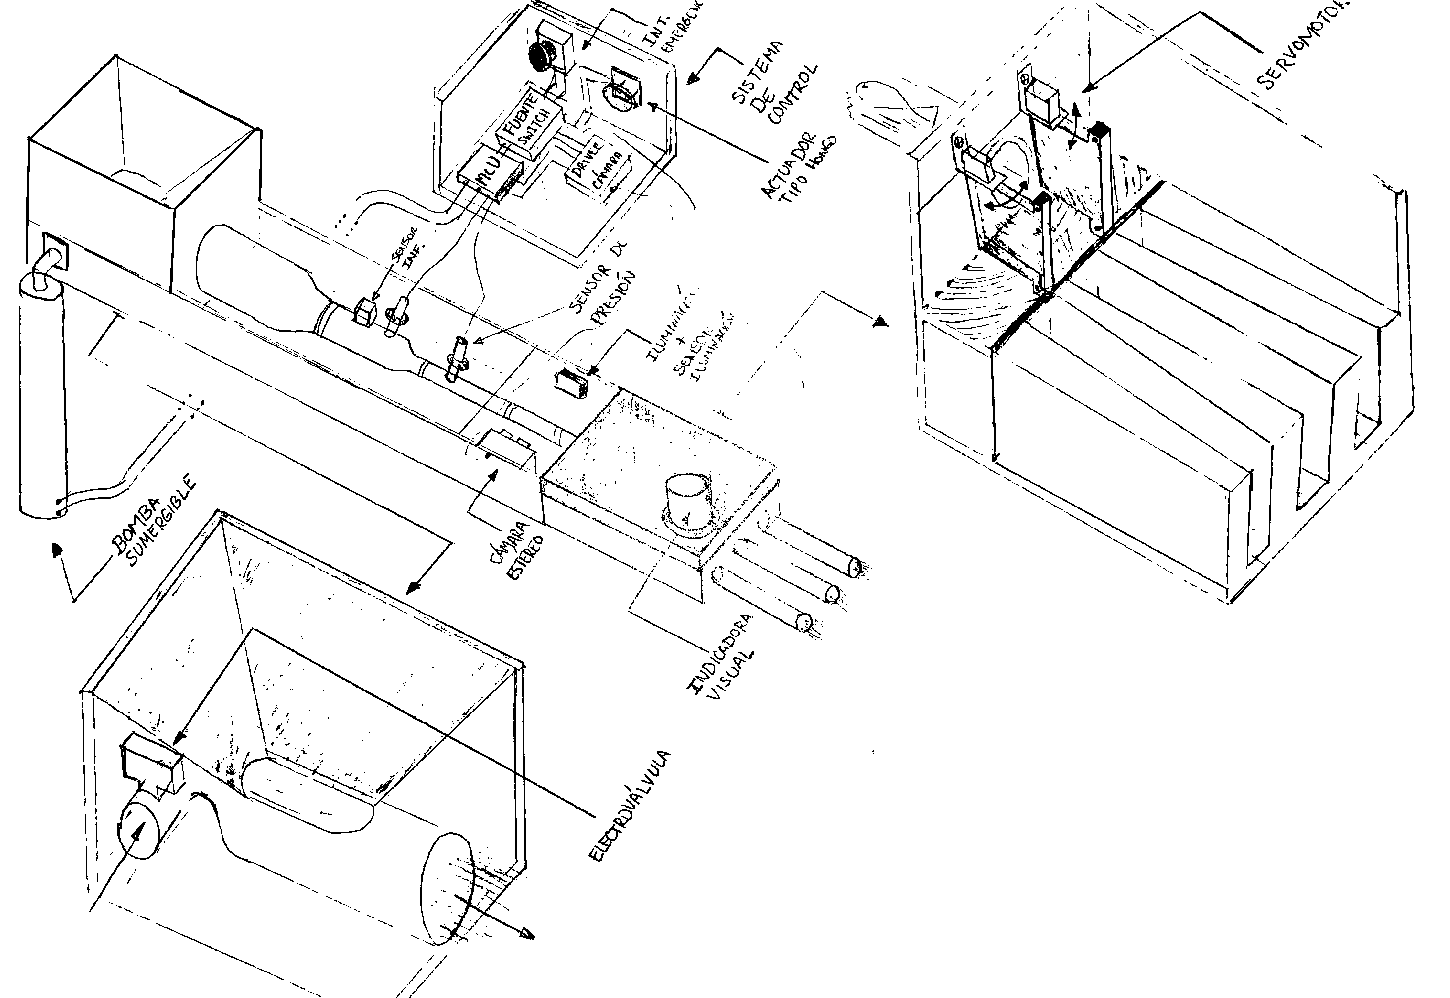
\includegraphics[width=0.85\textwidth]{chapter3/dibujo de concepto de solucion 2.png}
	\caption{Dibujo de concepto de solución N° 2.}
	Fuente: Elaboración propia.
	\label{fig:dibujo de concepto de solucion 2}
\end{figure}

%% NUEVA SUB-SUB-SECCION X.X.X.X
\subsubsection{Concepto de solución N° 3}

El tercer concepto de solución (Figura \ref{fig:dibujo de concepto de solucion 3}) hace uso de una plataforma flotante y una estructura como soporte para el sistema. En el dibujo se ha omitido los mecanismos que mantienen a flote a la plataforma. La preparación de este sistema la realiza un operario que revisa las tuberías y que no existan objetos que impidan el tránsito de las truchas. Primero el operario revisa si el botón de emergencia está activado, en caso contrario procede a encender el sistema mediante un interruptor posicionado en el sistema de control (parte lateral del sistema de recepción). Se conecta el teléfono inteligente de forma inalámbrica. El sistema realiza una prueba de los sensores para verificar un correcto funcionamiento. Luego de la verificación, mediante la aplicación se indica una cantidad de flujo deseada y el sistema se encarga de regularla.

\begin{figure}[H]
	\centering
	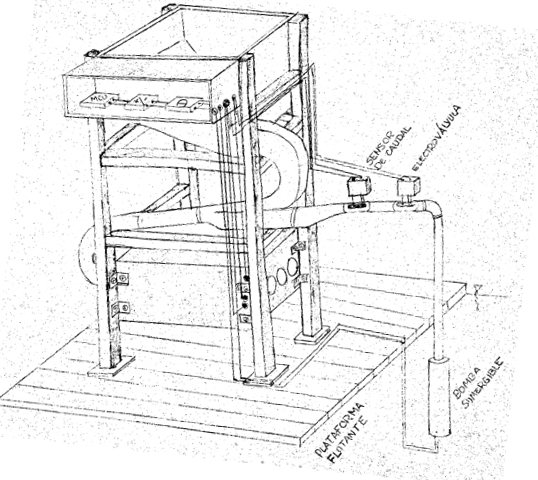
\includegraphics[width=0.75\textwidth]{chapter3/dibujo de concepto de solucion 3.png}
	\caption{Dibujo de concepto de solución N° 3.}
	Fuente: Elaboración propia.
	\label{fig:dibujo de concepto de solucion 3}
\end{figure}

Después, las truchas son depositas por la parte superior en el sistema físico de "recepción" de tal forma que solo puede pasar una por vez. Debido a la gravedad las truchas descenderán por la tubería hasta una parte dónde se le agrega caudal al sistema mediante un codo tipo "y griega" de tubería. A continuación, la trucha es medida y contada respecto a su clasificación. El sistema reporta a una aplicación móvil dicha información y controla las compuertas (Figura \ref{fig:dibujo de distribucion de truchas}) para direccionar a la trucha a la salida correspondiente. El sistema de distribución de truchas  de la Figura \ref{dibujo de concepto de solucion 3} es similar al del concepto solución N° 2, también se muestra en la Figura \ref{dibujo de distribucion de truchas}.

\begin{figure}[H]
	\centering
	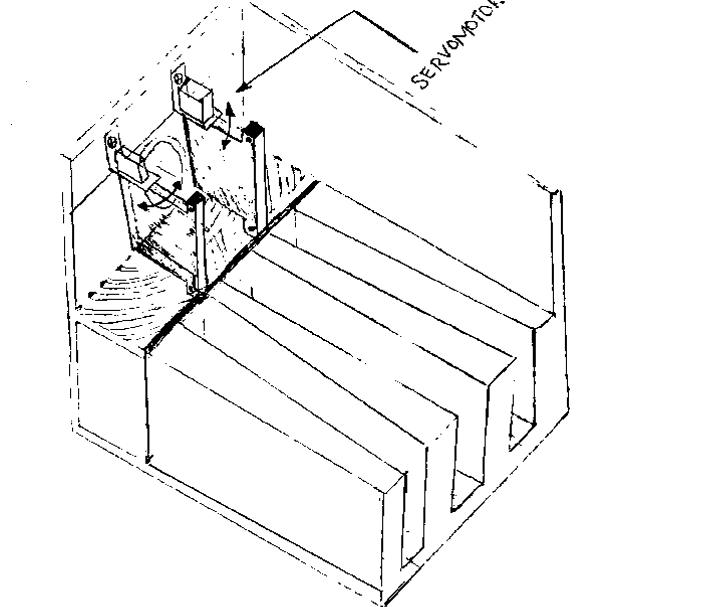
\includegraphics[width=0.45\textwidth]{chapter3/dibujo de distribucion de truchas.png}
	\caption{Dibujo de distribución de truchas.}
	Fuente: Elaboración propia.
	\label{fig:dibujo de distribucion de truchas}
\end{figure}

%% NUEVO SUBSECCION X.X.X
\subsection{Evaluación técnico-económica}

La evaluación de los conceptos se realiza tomando en cuenta diferentes criterios tanto cuantitativos como cualitativos. En la tabla Tabla \ref{tab:pesos de relevancia} se muestra la valoración y su significado.

% Please add the following required packages to your document preamble:
% \usepackage[table,xcdraw]{xcolor}
% If you use beamer only pass "xcolor=table" option, i.e. \documentclass[xcolor=table]{beamer}
\begin{table}[H]
	\centering
	\caption{Pesos de relevancia.}
	\label{tab:pesos de relevancia}
	\begin{tabular}{|c|c|}
		\hline
		\rowcolor[HTML]{D9D9D9} 
		\textbf{Valor (g)} & \textbf{Significado} \\ \hline
		4                  & Muy Importante       \\ \hline
		3                  & Importante           \\ \hline
		2                  & Indiferente          \\ \hline
		1                  & Poco Importante      \\ \hline
		0                  & Nada Importante      \\ \hline
	\end{tabular}
	\\Fuente: Elaboración propia.
\end{table}


Asimismo, cada concepto de solución planteado recibe el respectivo puntaje que indica qué tanto cumple con cada criterio. El puntaje y su significado se muestra en la Tabla \ref{tab:escala de efectividad de las soluciones}.

% Please add the following required packages to your document preamble:
% \usepackage[table,xcdraw]{xcolor}
% If you use beamer only pass "xcolor=table" option, i.e. \documentclass[xcolor=table]{beamer}
\begin{table}[H]
	\centering
	\caption{Escala de efectividad de las soluciones.}
	\label{tab:escala de efectividad de las soluciones}
	\begin{tabular}{|c|c|}
		\hline
		\rowcolor[HTML]{D9D9D9} 
		\textbf{Valor (g)} & \textbf{Significado} 					\\ \hline
		4                  & Satisface completamente (Ideal)        \\ \hline
		3                  & Satisface bien           				\\ \hline
		2                  & Satisface suficientemente        		\\ \hline
		1                  & Satisface infinitamente     			\\ \hline
		0                  & No satisface				     		\\ \hline
	\end{tabular}
	\\Fuente: Elaboración propia.
\end{table}


%% NUEVA SUB-SUB-SECCION X.X.X.X
\subsubsection{Criterios técnicos}

Los criterios técnicos escogidos para calificar el sistema son: \textbf{confiabilidad}, referido a alguna fuga de truchas en las tuberías o compartimientos que se puedan dar y que terminen liberando a la trucha al medio, \textbf{transportabilidad}, referido a la cantidad de pasos para poder ensamblar el sistema para poder usarlo y la dificultad de transportarlo de un lugar de almacenamiento hasta la jaula flotan-te en la situación mostrada en la Figura \ref{fig:dibujo conceptual de la problematica}; \textbf{complejidad}, referido al número de componentes, sensores y actuadores que emplea el sistema para cumplir su función; \textbf{uso de energía}, referido al consumo eléctrico de los sensores y actuadores que emplea el sistema para cumplir su función; \textbf{dimensiones}, referido a las dimensiones físicas del sistema en general.

% Please add the following required packages to your document preamble:
% \usepackage[table,xcdraw]{xcolor}
% If you use beamer only pass "xcolor=table" option, i.e. \documentclass[xcolor=table]{beamer}
\begin{table}[H]
	\centering
	\caption{Evaluación de criterios técnicos.}
	\label{tab:evaluacion de criterios tecnicos}
	\begin{tabular}{|
			>{\columncolor[HTML]{D9D9D9}}l |
			>{\columncolor[HTML]{D9D9D9}}l |
			>{\columncolor[HTML]{D9D9D9}}c |c|
			>{\columncolor[HTML]{D9D9D9}}c |c|
			>{\columncolor[HTML]{D9D9D9}}c |c|
			>{\columncolor[HTML]{D9D9D9}}c |c|
			>{\columncolor[HTML]{D9D9D9}}c |}
		\hline
		\multicolumn{3}{|c|}{\cellcolor[HTML]{A6A6A6}{\color[HTML]{000000} \textbf{Técnicos}}} &
		\multicolumn{2}{c|}{\cellcolor[HTML]{A6A6A6}{\color[HTML]{000000} \textbf{Solución 1}}} &
		\multicolumn{2}{c|}{\cellcolor[HTML]{A6A6A6}{\color[HTML]{000000} \textbf{Solución 2}}} &
		\multicolumn{2}{c|}{\cellcolor[HTML]{A6A6A6}{\color[HTML]{000000} \textbf{Solución 3}}} &
		\multicolumn{2}{c|}{\cellcolor[HTML]{A6A6A6}{\color[HTML]{000000} \textbf{Solución ideal}}} \\ \hline
		\multicolumn{1}{|c|}{\cellcolor[HTML]{A6A6A6}{\color[HTML]{000000} \textbf{N°}}} &
		\multicolumn{1}{c|}{\cellcolor[HTML]{A6A6A6}{\color[HTML]{000000} \textbf{Criterio}}} &
		\cellcolor[HTML]{A6A6A6}{\color[HTML]{000000} \textbf{g}} &
		\cellcolor[HTML]{A6A6A6}{\color[HTML]{000000} \textbf{p}} &
		\cellcolor[HTML]{A6A6A6}{\color[HTML]{000000} \textbf{pxg}} &
		\cellcolor[HTML]{A6A6A6}{\color[HTML]{000000} \textbf{p}} &
		\cellcolor[HTML]{A6A6A6}{\color[HTML]{000000} \textbf{pxg}} &
		\cellcolor[HTML]{A6A6A6}{\color[HTML]{000000} \textbf{p}} &
		\cellcolor[HTML]{A6A6A6}{\color[HTML]{000000} \textbf{pxg}} &
		\cellcolor[HTML]{A6A6A6}{\color[HTML]{000000} \textbf{p}} &
		\cellcolor[HTML]{A6A6A6}{\color[HTML]{000000} \textbf{pxg}} \\ \hline
		{\color[HTML]{000000} 1} &
		{\color[HTML]{000000} Confiabilidad} &
		{\color[HTML]{000000} 3} &
		{\color[HTML]{000000} 2} &
		{\color[HTML]{000000} 6} &
		{\color[HTML]{000000} 3} &
		{\color[HTML]{000000} 9} &
		{\color[HTML]{000000} 2} &
		{\color[HTML]{000000} 6} &
		{\color[HTML]{000000} 4} &
		{\color[HTML]{000000} 12} \\ \hline
		{\color[HTML]{000000} 2} &
		{\color[HTML]{000000} Transportabilidad} &
		{\color[HTML]{000000} 4} &
		{\color[HTML]{000000} 2} &
		{\color[HTML]{000000} 8} &
		{\color[HTML]{000000} 3} &
		{\color[HTML]{000000} 12} &
		{\color[HTML]{000000} 2} &
		{\color[HTML]{000000} 8} &
		{\color[HTML]{000000} 4} &
		{\color[HTML]{000000} 16} \\ \hline
		{\color[HTML]{000000} 3} &
		{\color[HTML]{000000} Complejidad} &
		{\color[HTML]{000000} 3} &
		{\color[HTML]{000000} 3} &
		{\color[HTML]{000000} 9} &
		{\color[HTML]{000000} 3} &
		{\color[HTML]{000000} 9} &
		{\color[HTML]{000000} 2} &
		{\color[HTML]{000000} 6} &
		{\color[HTML]{000000} 4} &
		{\color[HTML]{000000} 12} \\ \hline
		{\color[HTML]{000000} 4} &
		{\color[HTML]{000000} Uso de energía} &
		{\color[HTML]{000000} 2} &
		{\color[HTML]{000000} 1} &
		{\color[HTML]{000000} 2} &
		{\color[HTML]{000000} 3} &
		{\color[HTML]{000000} 6} &
		{\color[HTML]{000000} 2} &
		{\color[HTML]{000000} 4} &
		{\color[HTML]{000000} 4} &
		{\color[HTML]{000000} 8} \\ \hline
		{\color[HTML]{000000} 5} &
		{\color[HTML]{000000} Dimensiones} &
		{\color[HTML]{000000} 3} &
		{\color[HTML]{000000} 2} &
		{\color[HTML]{000000} 6} &
		{\color[HTML]{000000} 2} &
		{\color[HTML]{000000} 6} &
		{\color[HTML]{000000} 3} &
		{\color[HTML]{000000} 9} &
		{\color[HTML]{000000} 4} &
		{\color[HTML]{000000} 12} \\ \hline
		\multicolumn{3}{|l|}{\cellcolor[HTML]{A6A6A6}{\color[HTML]{000000} \textbf{Suma}}} &
		\cellcolor[HTML]{D9D9D9}{\color[HTML]{000000} 10} &
		{\color[HTML]{000000} 31} &
		\cellcolor[HTML]{D9D9D9}{\color[HTML]{000000} 14} &
		{\color[HTML]{000000} 42} &
		\cellcolor[HTML]{D9D9D9}{\color[HTML]{000000} 11} &
		{\color[HTML]{000000} 33} &
		\cellcolor[HTML]{D9D9D9}{\color[HTML]{000000} 20} &
		{\color[HTML]{000000} 60} \\ \hline
		\multicolumn{3}{|l|}{\cellcolor[HTML]{A6A6A6}{\color[HTML]{000000} \textbf{Promedio ponderado}}} &
		\cellcolor[HTML]{D9D9D9}{\color[HTML]{000000} \textbf{0.50}} &
		\cellcolor[HTML]{A6A6A6}{\color[HTML]{000000} \textbf{0.52}} &
		\cellcolor[HTML]{D9D9D9}{\color[HTML]{000000} \textbf{0.70}} &
		\cellcolor[HTML]{A6A6A6}{\color[HTML]{000000} \textbf{0.70}} &
		\cellcolor[HTML]{D9D9D9}{\color[HTML]{000000} \textbf{0.55}} &
		\cellcolor[HTML]{A6A6A6}{\color[HTML]{000000} \textbf{0.55}} &
		\cellcolor[HTML]{D9D9D9}{\color[HTML]{000000} \textbf{1.0}} &
		\cellcolor[HTML]{A6A6A6}{\color[HTML]{000000} \textbf{1.0}} \\ \hline
	\end{tabular}
	\\ Fuente: Elaboración propia.
\end{table}

%% NUEVA SUB-SUB-SECCION X.X.X.X
\subsubsection{Criterios económicos}

Los criterios económicos escogidos para calificar el sistema son: \textbf{número de piezas}, referido a la cantidad de componentes electrónicos que emplea el concepto para cumplir las funciones; \textbf{costo de piezas}, referido al costo de adquisición de los componentes electrónicos y mecánicos; \textbf{productividad}, referido a la cantidad de truchas que puede procesar el sistema; fácil montaje, referido al tiempo que toma ensamblar el sistema para poder usarlo; \textbf{fácil adquisición}, referido a la existencia en stock de los materiales de fabricación para poder hacer el sistema.

% Please add the following required packages to your document preamble:
% \usepackage[table,xcdraw]{xcolor}
% If you use beamer only pass "xcolor=table" option, i.e. \documentclass[xcolor=table]{beamer}
\begin{table}[H]
	\centering
	\caption{Evaluación de criterios económicos.}
	\label{tab:evaluacion de criterios economicos}
	\begin{tabular}{|
			>{\columncolor[HTML]{D9D9D9}}c |
			>{\columncolor[HTML]{D9D9D9}}l |
			>{\columncolor[HTML]{D9D9D9}}c |c|
			>{\columncolor[HTML]{D9D9D9}}c |c|
			>{\columncolor[HTML]{D9D9D9}}c |c|
			>{\columncolor[HTML]{D9D9D9}}c |c|
			>{\columncolor[HTML]{D9D9D9}}c |}
		\hline
		\multicolumn{3}{|c|}{\cellcolor[HTML]{A6A6A6}{\color[HTML]{000000} \textbf{Técnicos}}} &
		\multicolumn{2}{c|}{\cellcolor[HTML]{A6A6A6}{\color[HTML]{000000} \textbf{Solución 1}}} &
		\multicolumn{2}{c|}{\cellcolor[HTML]{A6A6A6}{\color[HTML]{000000} \textbf{Solución 2}}} &
		\multicolumn{2}{c|}{\cellcolor[HTML]{A6A6A6}{\color[HTML]{000000} \textbf{Solución 3}}} &
		\multicolumn{2}{c|}{\cellcolor[HTML]{A6A6A6}{\color[HTML]{000000} \textbf{Solución ideal}}} \\ \hline
		\cellcolor[HTML]{A6A6A6}{\color[HTML]{000000} \textbf{N°}} &
		\multicolumn{1}{c|}{\cellcolor[HTML]{A6A6A6}{\color[HTML]{000000} \textbf{Criterio}}} &
		\cellcolor[HTML]{A6A6A6}{\color[HTML]{000000} \textbf{g}} &
		\cellcolor[HTML]{A6A6A6}{\color[HTML]{000000} \textbf{p}} &
		\cellcolor[HTML]{A6A6A6}{\color[HTML]{000000} \textbf{pxg}} &
		\cellcolor[HTML]{A6A6A6}{\color[HTML]{000000} \textbf{p}} &
		\cellcolor[HTML]{A6A6A6}{\color[HTML]{000000} \textbf{pxg}} &
		\cellcolor[HTML]{A6A6A6}{\color[HTML]{000000} \textbf{p}} &
		\cellcolor[HTML]{A6A6A6}{\color[HTML]{000000} \textbf{pxg}} &
		\cellcolor[HTML]{A6A6A6}{\color[HTML]{000000} \textbf{p}} &
		\cellcolor[HTML]{A6A6A6}{\color[HTML]{000000} \textbf{pxg}} \\ \hline
		{\color[HTML]{000000} 1} &
		{\color[HTML]{000000} Número de piezas} &
		{\color[HTML]{000000} 3} &
		{\color[HTML]{000000} 2} &
		{\color[HTML]{000000} 6} &
		{\color[HTML]{000000} 3} &
		{\color[HTML]{000000} 9} &
		{\color[HTML]{000000} 3} &
		{\color[HTML]{000000} 9} &
		{\color[HTML]{000000} 4} &
		{\color[HTML]{000000} 12} \\ \hline
		{\color[HTML]{000000} 2} &
		{\color[HTML]{000000} Costo de piezas} &
		{\color[HTML]{000000} 4} &
		{\color[HTML]{000000} 3} &
		{\color[HTML]{000000} 12} &
		{\color[HTML]{000000} 3} &
		{\color[HTML]{000000} 12} &
		{\color[HTML]{000000} 2} &
		{\color[HTML]{000000} 8} &
		{\color[HTML]{000000} 4} &
		{\color[HTML]{000000} 16} \\ \hline
		{\color[HTML]{000000} 3} &
		{\color[HTML]{000000} Productividad} &
		{\color[HTML]{000000} 3} &
		{\color[HTML]{000000} 3} &
		{\color[HTML]{000000} 9} &
		{\color[HTML]{000000} 2} &
		{\color[HTML]{000000} 6} &
		{\color[HTML]{000000} 2} &
		{\color[HTML]{000000} 6} &
		{\color[HTML]{000000} 4} &
		{\color[HTML]{000000} 12} \\ \hline
		{\color[HTML]{000000} 4} &
		{\color[HTML]{000000} Fácil montaje} &
		{\color[HTML]{000000} 2} &
		{\color[HTML]{000000} 2} &
		{\color[HTML]{000000} 4} &
		{\color[HTML]{000000} 3} &
		{\color[HTML]{000000} 6} &
		{\color[HTML]{000000} 2} &
		{\color[HTML]{000000} 4} &
		{\color[HTML]{000000} 4} &
		{\color[HTML]{000000} 8} \\ \hline
		{\color[HTML]{000000} 5} &
		{\color[HTML]{000000} Fácil adquisición} &
		{\color[HTML]{000000} 4} &
		{\color[HTML]{000000} 3} &
		{\color[HTML]{000000} 12} &
		{\color[HTML]{000000} 3} &
		{\color[HTML]{000000} 12} &
		{\color[HTML]{000000} 2} &
		{\color[HTML]{000000} 8} &
		{\color[HTML]{000000} 4} &
		{\color[HTML]{000000} 16} \\ \hline
		\multicolumn{3}{|l|}{\cellcolor[HTML]{A6A6A6}{\color[HTML]{000000} \textbf{Suma}}} &
		\cellcolor[HTML]{D9D9D9}{\color[HTML]{000000} 13} &
		{\color[HTML]{000000} 43} &
		\cellcolor[HTML]{D9D9D9}{\color[HTML]{000000} 14} &
		{\color[HTML]{000000} 45} &
		\cellcolor[HTML]{D9D9D9}{\color[HTML]{000000} 11} &
		{\color[HTML]{000000} 35} &
		\cellcolor[HTML]{D9D9D9}{\color[HTML]{000000} 20} &
		{\color[HTML]{000000} 64} \\ \hline
		\multicolumn{3}{|l|}{\cellcolor[HTML]{A6A6A6}{\color[HTML]{000000} \textbf{Promedio ponderado}}} &
		\cellcolor[HTML]{D9D9D9}{\color[HTML]{000000} \textbf{0.65}} &
		\cellcolor[HTML]{A6A6A6}{\color[HTML]{000000} \textbf{0.67}} &
		\cellcolor[HTML]{D9D9D9}{\color[HTML]{000000} \textbf{0.70}} &
		\cellcolor[HTML]{A6A6A6}{\color[HTML]{000000} \textbf{0.71}} &
		\cellcolor[HTML]{D9D9D9}{\color[HTML]{000000} \textbf{0.55}} &
		\cellcolor[HTML]{A6A6A6}{\color[HTML]{000000} \textbf{0.54}} &
		\cellcolor[HTML]{D9D9D9}{\color[HTML]{000000} \textbf{1.0}} &
		\cellcolor[HTML]{A6A6A6}{\color[HTML]{000000} \textbf{1.0}} \\ \hline
	\end{tabular}
	\\ Fuente: Elaboración propia.
\end{table}

%% NUEVA SUB-SUB-SECCION X.X.X.X
\subsubsection{Elección de concepto óptimo}

Con los datos obtenidos en la Tabla \ref{tab:evaluacion de criterios tecnicos} y Tabla \ref{tab:evaluacion de criterios economicos} podemos hacer una comparación numérica de promedios ponderados de valoraciones según criterios establecidos. En la Figura \ref{fig:analisis tecnico economico} se muestra esta comparación en un gráfico de dispersión, en la que el eje vertical es el valor obtenido de cada solución en los criterios técnicos y en el caso del eje horizontal es el valor obtenido en cada solución en los criterios económicos.

\begin{figure}[H]
	\centering
	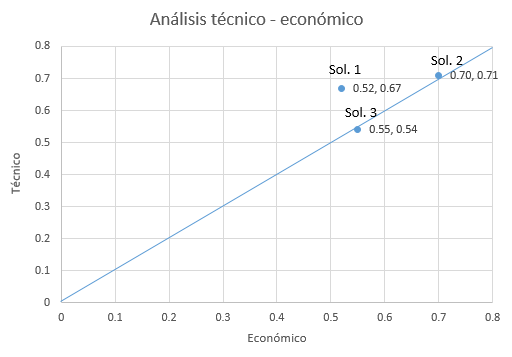
\includegraphics[width=0.75\textwidth]{chapter3/analisis tecnico economico.png}
	\caption{Análisis técnico económico.}
	Fuente: Elaboración propia.
	\label{fig:analisis tecnico economico}
\end{figure}

El \textbf{concepto de solución N° 2 obtuvo un mejor puntaje} con respecto a las otras dos alternativas por lo cual se selecciona como la \textbf{propuesta óptima}. Además, muestra un equilibrio entre la valoración técnica y económica. Por lo que se escoge este concepto de solución como solución óptima.

%% NUEVO SUBSECCION X.X.X
\subsection{Diagrama de operaciones de solución seleccionada}

El diagrama de operaciones muestra la secuencia de pasos para poder operar la máquina o sistema de forma adecuada en un funcionamiento normal. En la Figura \ref{fig:proceso de clasificacion y conteo manual} se muestra a modo de referencia el diagrama de operaciones del proceso manual, la Figura \ref{fig:proceso de clasificacion y conteo propuesto} muestra el método propuesto y la secuencia de acciones se explaya en la Figura \ref{fig:flujograma de funcionamiento de la solucion optima}.

\newpage
\pagestyle{mylandscape}

\begin{landscape}
	\begin{figure}[H]
		\centering
		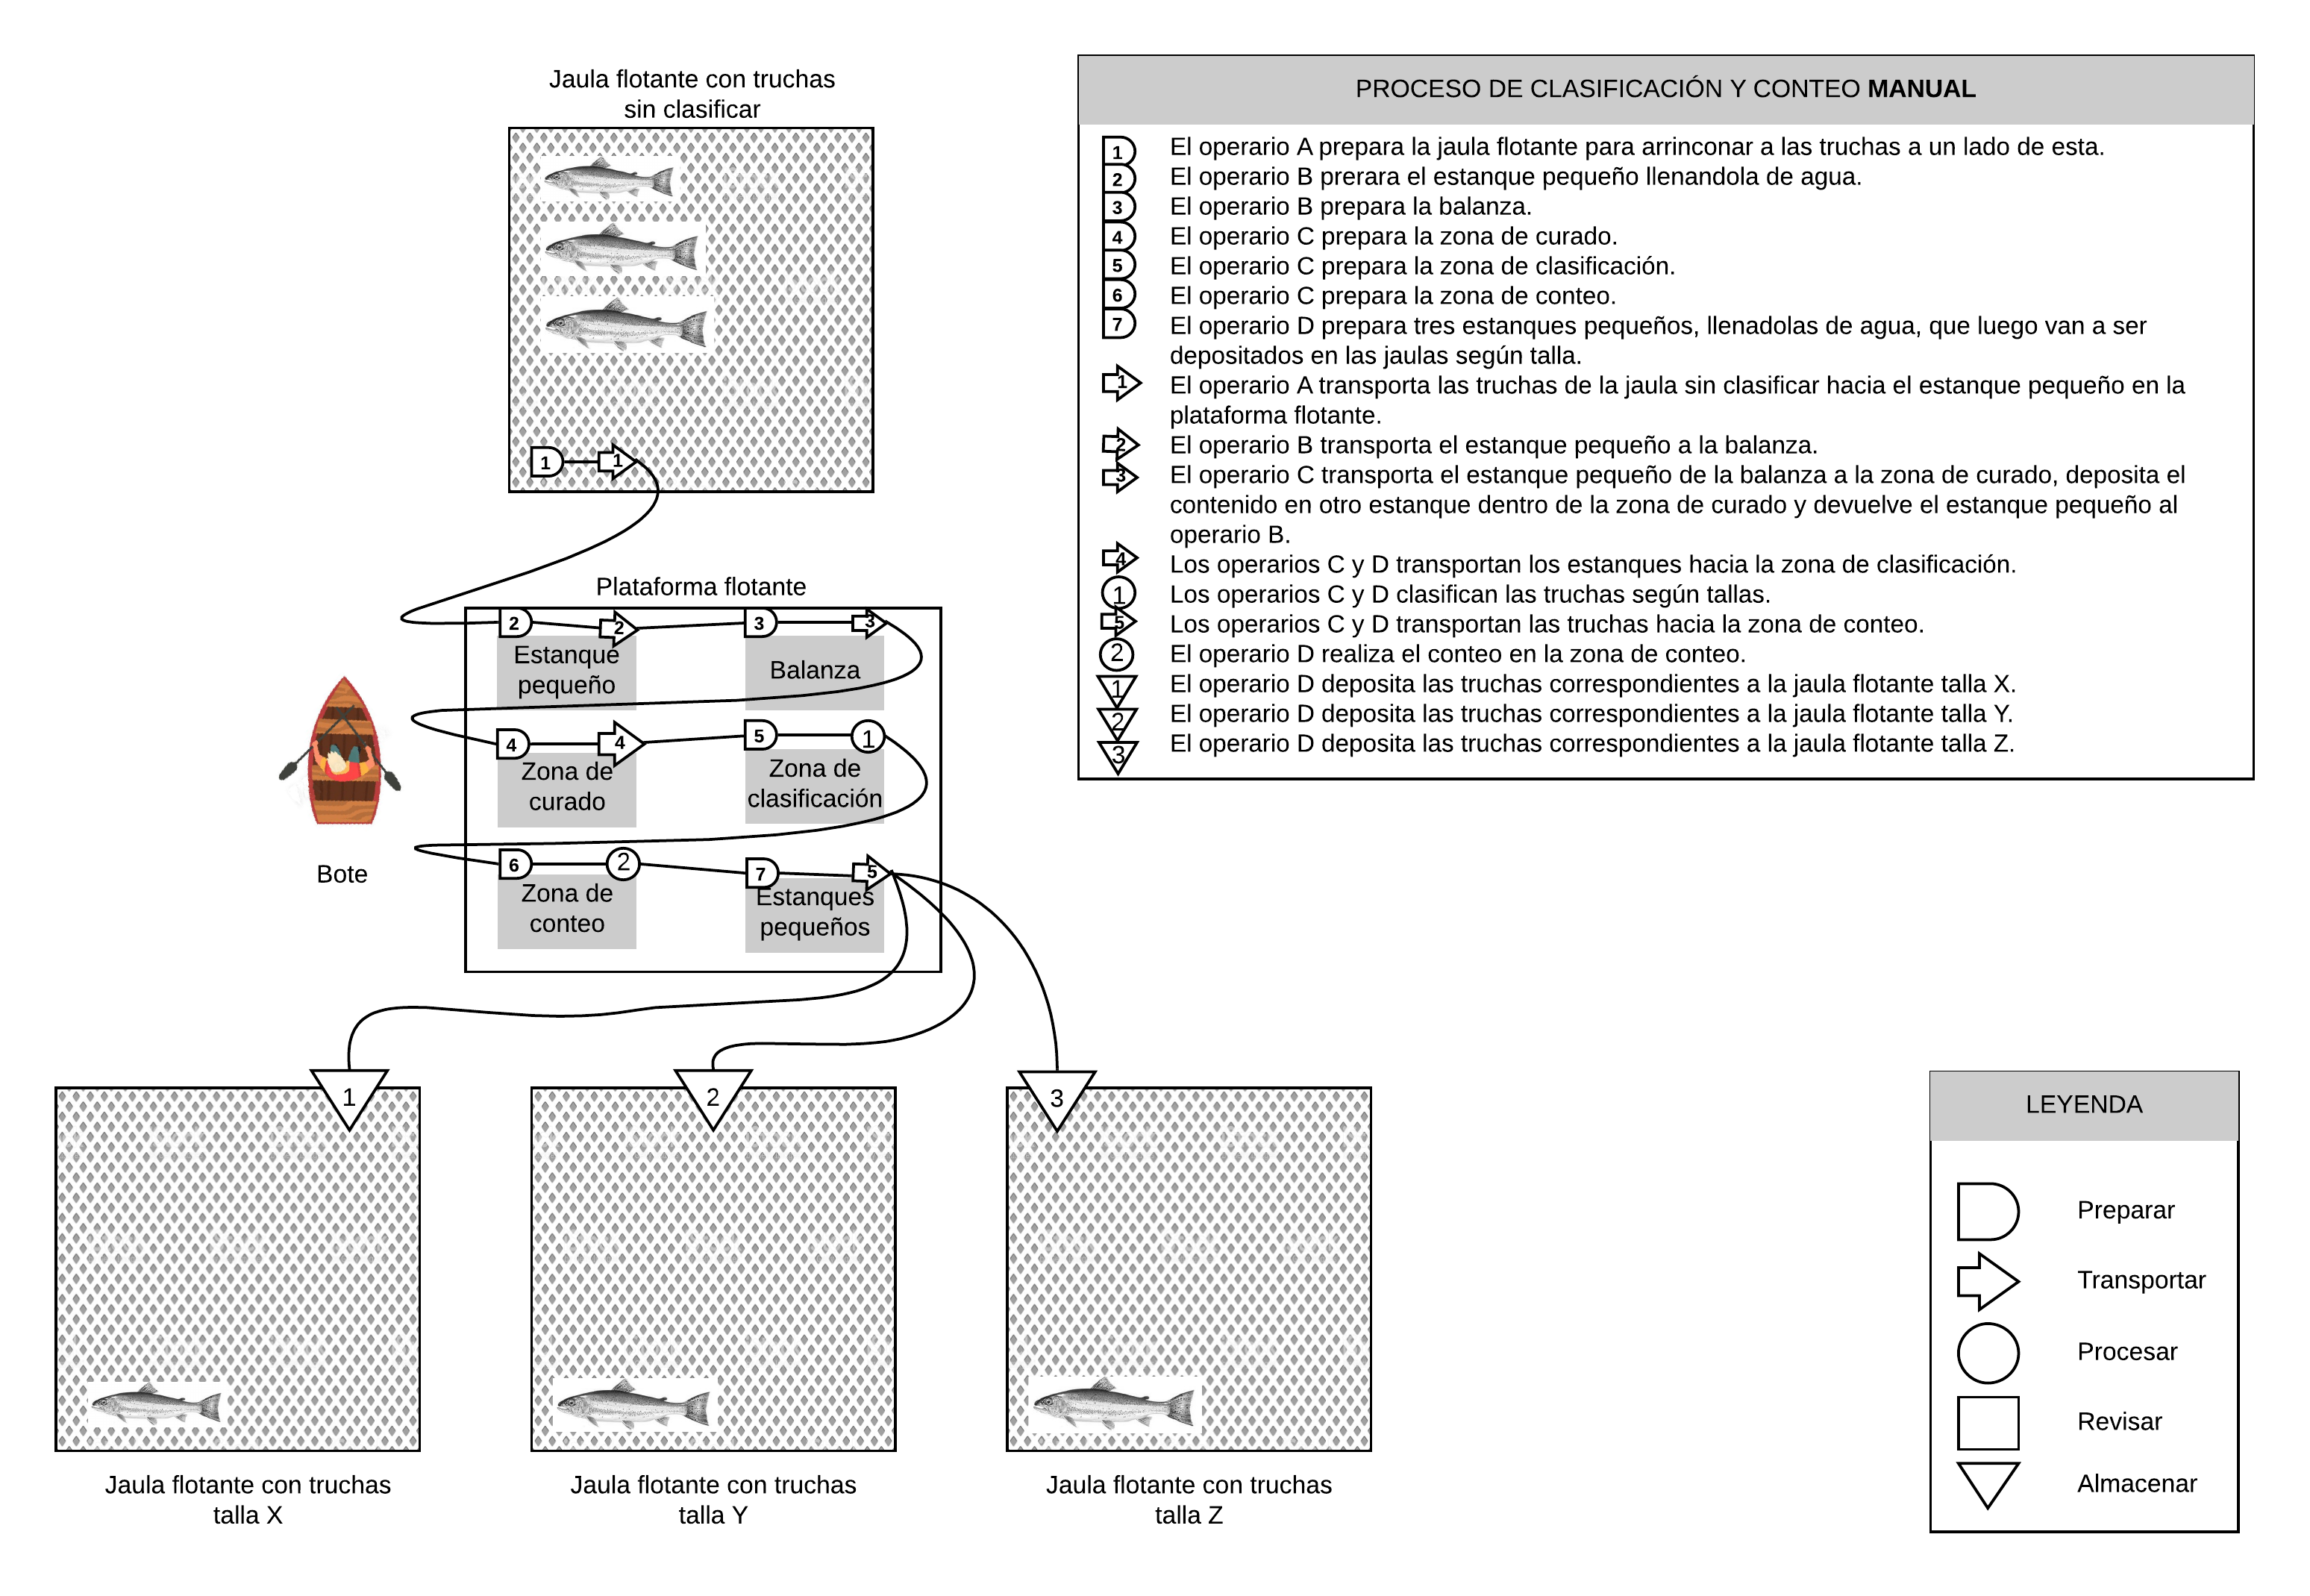
\includegraphics[width=0.98\paperwidth]{chapter3/proceso de clasificacion y conteo manual.png}
		\caption{Método manual de clasificación y conteo de truchas.}
		Fuente: Elaboración propia.
		\label{fig:proceso de clasificacion y conteo manual}
	\end{figure}
\end{landscape}

\begin{landscape}
	\begin{figure}[H]
		\centering
		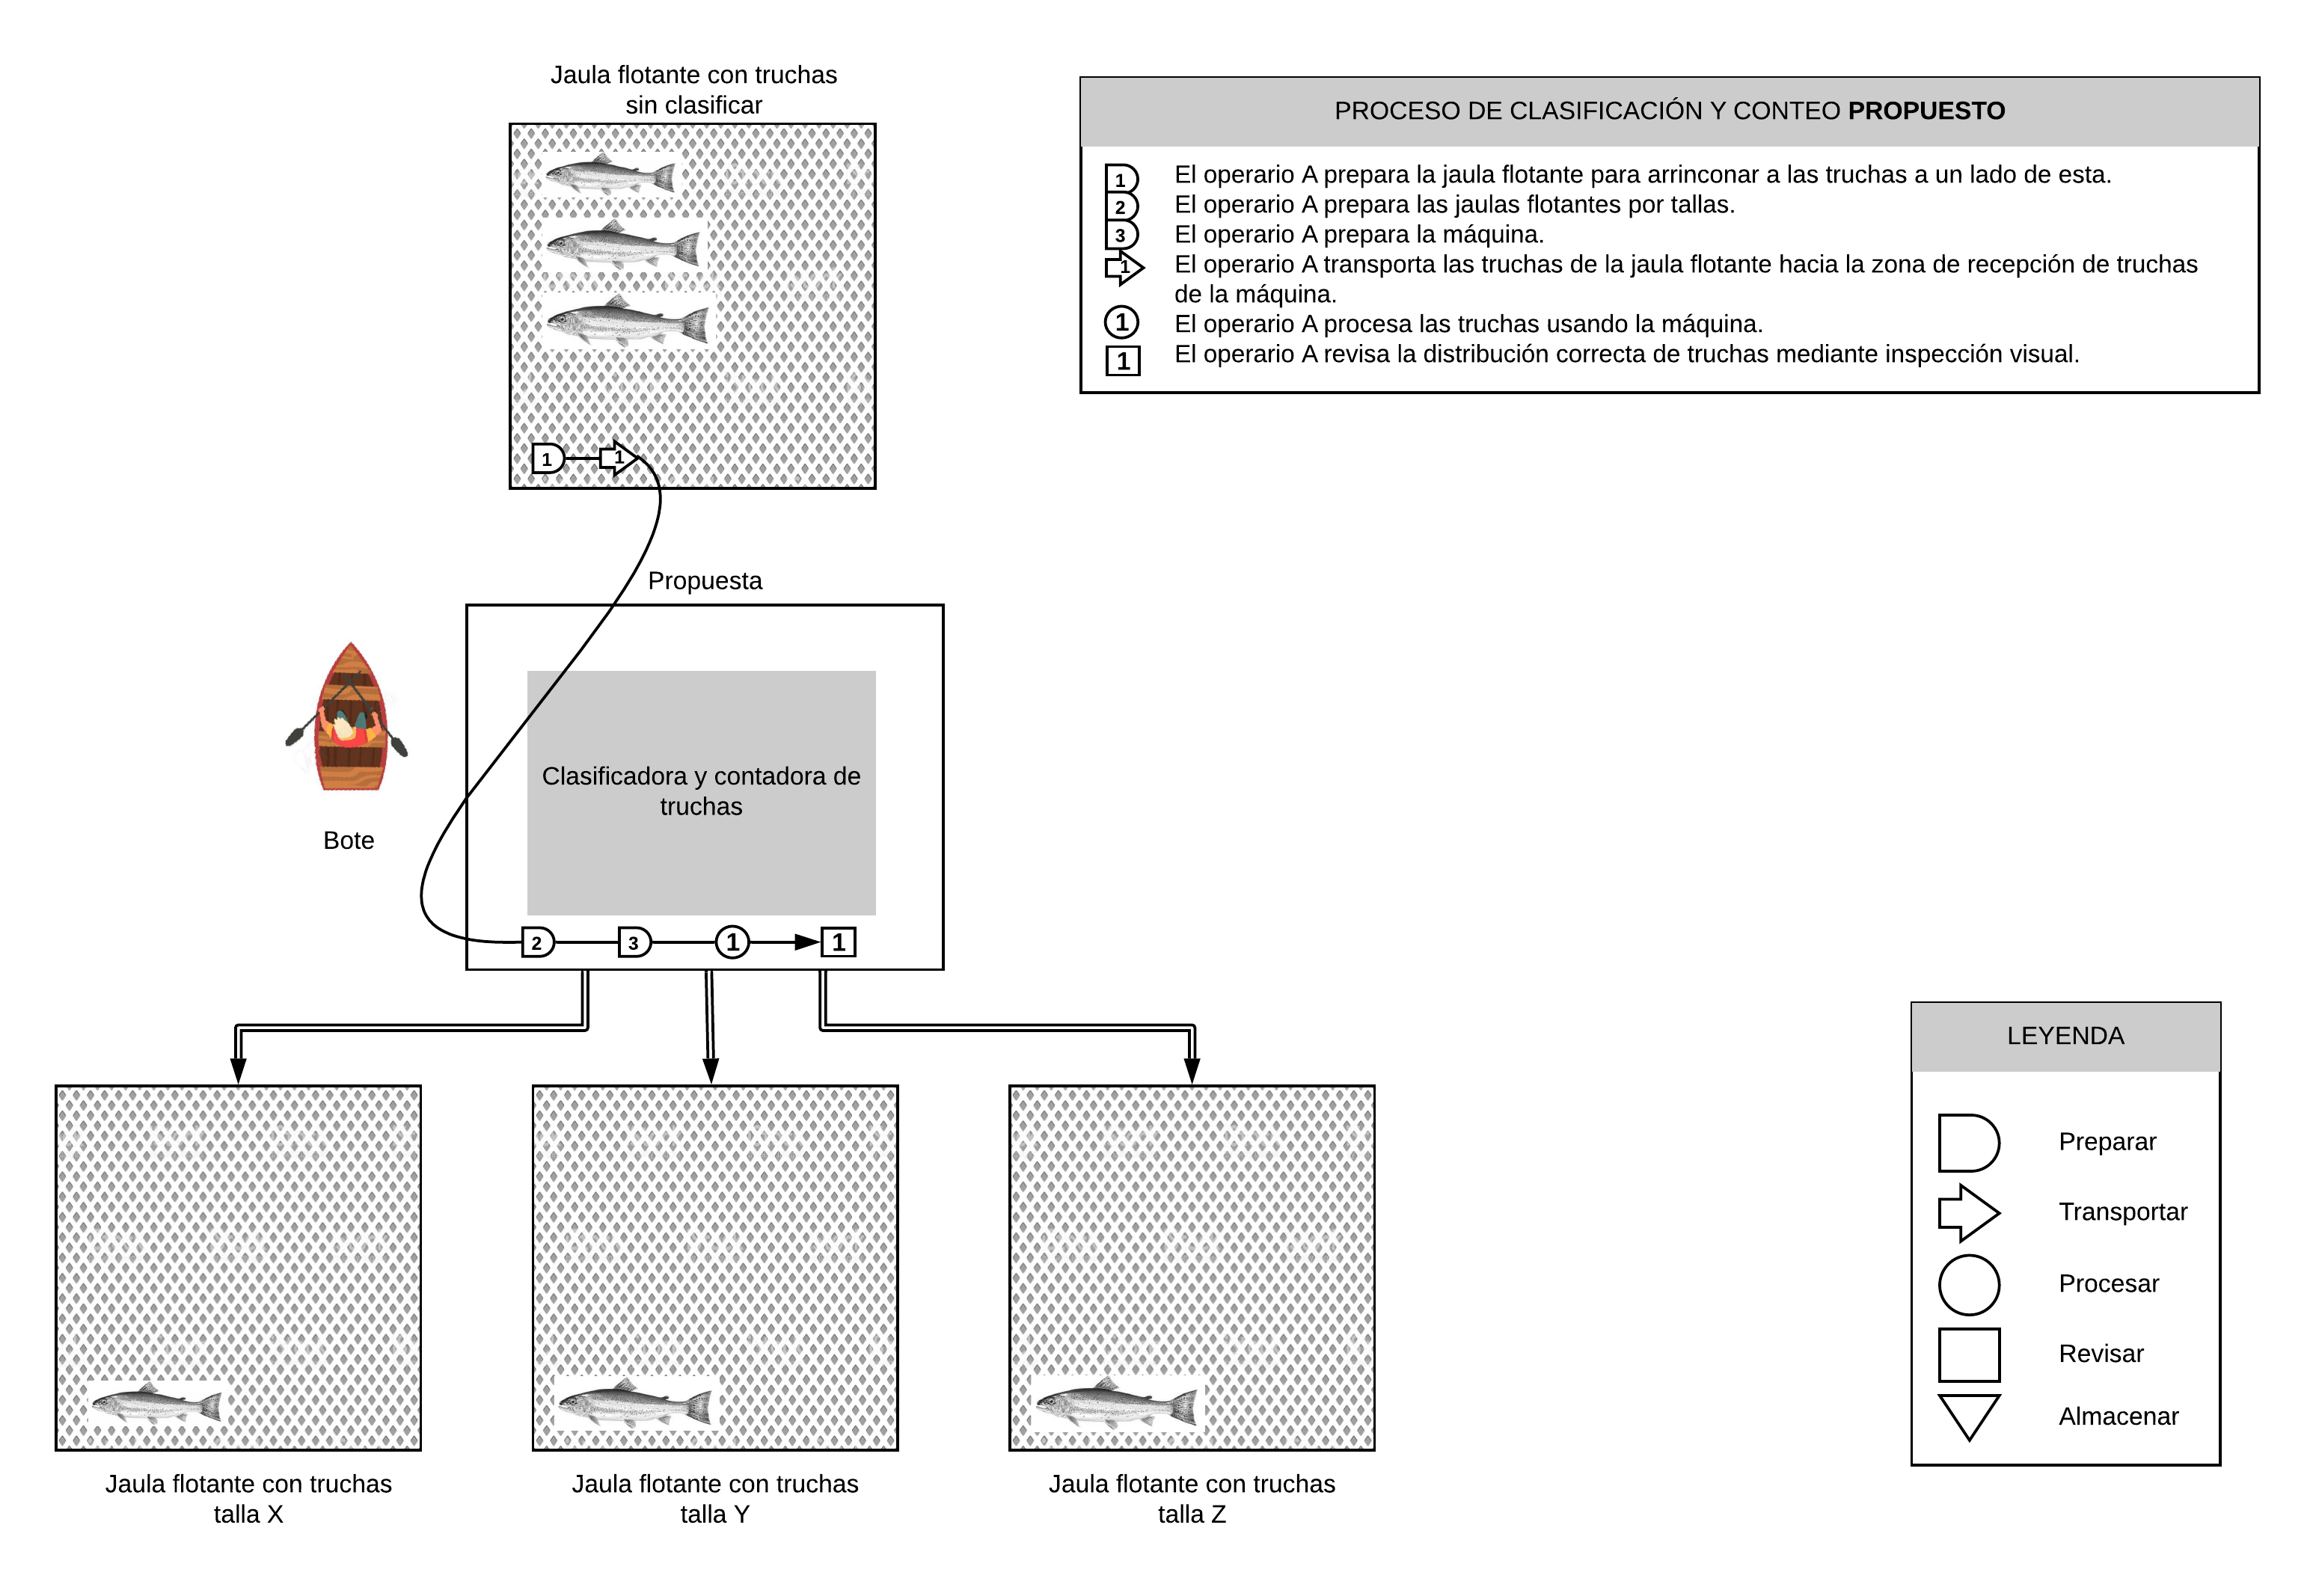
\includegraphics[width=0.98\paperwidth]{chapter3/proceso de clasificacion y conteo propuesto.png}
		\caption{Método propuesto de clasificación y conteo de truchas.}
		Fuente: Elaboración propia.
		\label{fig:proceso de clasificacion y conteo propuesto}
	\end{figure}
\end{landscape}

\begin{landscape}
	\begin{figure}[H]
		\centering
		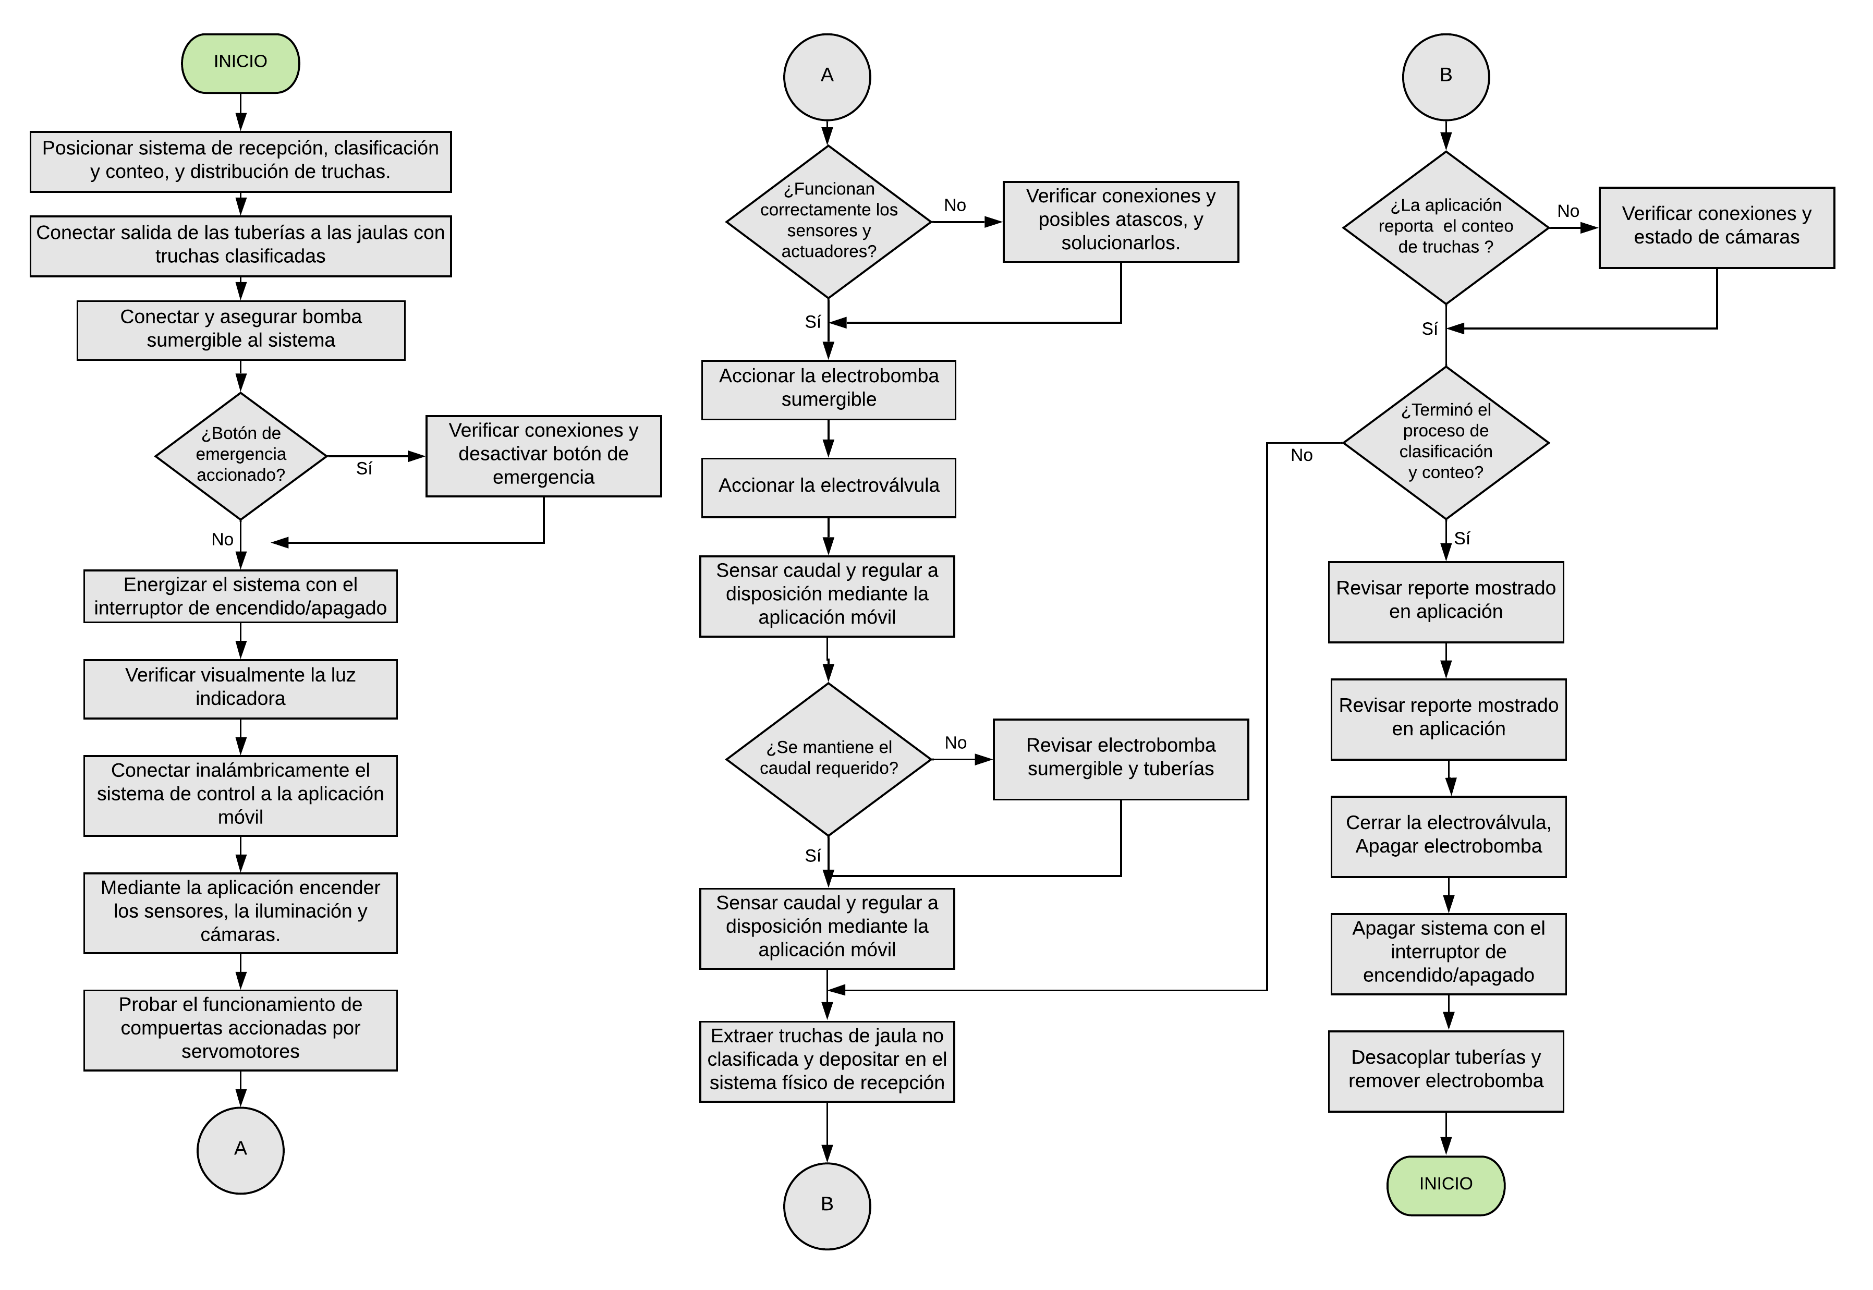
\includegraphics[width=0.98\paperwidth]{chapter3/flujograma de funcionamiento de la solucion optima.png}
		\caption{Flujograma de funcionamiento de la solución óptima.}
		Fuente: Elaboración propia.
		\label{fig:flujograma de funcionamiento de la solucion optima}
	\end{figure}
\end{landscape}







%%%%%%% FALTA PUNTOS 
%%%%%%% FALTA PUNTOS 
%%%%%%% FALTA PUNTOS 
%%%%%%% FALTA PUNTOS 
%%%%%%% FALTA PUNTOS 
%%%%%%% FALTA PUNTOS 
%%%%%%% FALTA PUNTOS 
%%%%%%% FALTA PUNTOS 




